\documentclass[conference]{IEEEtran}
\IEEEoverridecommandlockouts
\usepackage{cite}
\usepackage{amsmath,amssymb,amsfonts}
\usepackage{graphicx}
\usepackage{textcomp}
\usepackage{xcolor}
\usepackage{booktabs}
\usepackage{tabularx}
\usepackage{multirow}
\usepackage{array}
\usepackage{threeparttable}
\usepackage{stfloats}
\usepackage{url}
\usepackage{tikz}
\usetikzlibrary{positioning,arrows.meta,fit,shapes.geometric}

\graphicspath{{../results/}}
\renewcommand{\ttdefault}{cmtt}
\newcommand{\km}{\,km}
\newcommand{\m}{\,m}

\begin{document}

\title{Auditing the RTE Compliance Gap: Network-Based Geospatial Analysis of Walking Access to Government Schools in Bengaluru's Formal and Informal Settlements}

\author{\IEEEauthorblockN{Kaveri Sharma}
\IEEEauthorblockA{\textit{Dept. of Computer Science Engg.} \\
\textit{PES University}\\
Bengaluru, India \\
kaveri05sharma@gmail.com}
\and
\IEEEauthorblockN{Vedika Chhabra}
\IEEEauthorblockA{\textit{Dept. of Computer Science Engg.} \\
\textit{PES University}\\
Bengaluru, India \\
vedikac11@gmail.com}
\and
\IEEEauthorblockN{Jahnvi R}
\IEEEauthorblockA{\textit{Dept. of Computer Science Engg.} \\
\textit{PES University}\\
Bengaluru, India \\
jahnvi04@gmail.com}
\and
\IEEEauthorblockN{Manasa Ranganath}
\IEEEauthorblockA{\textit{Dept. of Computer Science Engg.} \\
\textit{PES University}\\
Bengaluru, India \\
manasaranganath06@gmail.com}
\and
\IEEEauthorblockN{Komal Kumari}
\IEEEauthorblockA{\textit{Dept. of Computer Science Engg.} \\
\textit{PES University}\\
Bengaluru, India \\
jaiswalkomal048@gmail.com}
\and
\IEEEauthorblockN{Dr. Divyashree N}
\IEEEauthorblockA{\textit{Associate Professor} \\
\textit{PES University}\\
Bengaluru, India \\
divyashreen@pes.edu}
}

\maketitle

\begin{abstract}
The Right of Children to Free and Compulsory Education (RTE) Act, 2009, and its rules require a government primary school within 1\km{} walking distance of every child's habitation. Compliance is usually audited with outdated census frames and straight-line (``crow-flies'') buffers, which are blind both to informal settlements and to the real street network. This paper presents an open, reproducible geospatial pipeline that audits RTE walking-distance compliance in Bengaluru. Sentinel-2 imagery and a Random Forest classifier delineate formal and informal built-up morphology; OpenStreetMap (OSM) supplies a 186,595-node pedestrian graph and 1,464 school features; and a single multi-source Dijkstra search, which partitions the street network into government-school catchments (a network Voronoi diagram), computes the exact network distance from 1,000 classified sample locations and all 509 Karnataka Slum Development Board (KSDB) slum polygons to the nearest government school. WorldPop 2020 population estimates weight every result. Using a curated set of 111 government schools, only 17.3\% of sampled locations and 20.1\% of the 226,753 slum residents lie within a 1\km{} walk. Planned layouts are on average 220\m{} farther than informal areas (2.32 vs.\ 2.10\km{}), but the difference is negligible in effect size (Cliff's $\delta=0.06$) and sensitive to how government schools are identified. Crow-flies buffers overstate compliance: 48.2\% of locations that appear compliant by straight line are non-compliant by network distance. Non-notified slums are significantly farther from government schools than notified slums (population-weighted 2.40 vs.\ 1.71\km{}; $p<10^{-5}$), and slum demand is highly concentrated: the ten most-loaded schools are the nearest government school for 71.5\% of slum residents (Gini $=0.85$). Meanwhile, 71--76\% of locations lie within 1\km{} of a non-government school. The results show that the compliance gap is city-wide, that it is underestimated by Euclidean audits, and that it falls hardest on settlements that are administratively invisible. Because OSM under-records government schools, all compliance figures are best read as lower bounds on access.
\end{abstract}

\begin{IEEEkeywords}
Right to Education, spatial accessibility, informal settlements, OpenStreetMap, OSMnx, network analysis, Dijkstra, Sentinel-2, Random Forest, WorldPop, Bengaluru.
\end{IEEEkeywords}

%=====================================================================
\section{Introduction}
%=====================================================================
\subsection{Problem Domain}
Bengaluru is one of the fastest-growing metropolitan regions in India. The 2011 Census recorded 8.44 million residents within the Bruhat Bengaluru Mahanagara Palike (BBMP) limits and 8.52 million in the urban agglomeration \cite{census2011}, and growth since then has been concentrated at the periphery, much of it unplanned. Rapid growth of this kind produces informal settlements whose boundaries, populations, and service needs are not reflected in the planning record for years \cite{unhabitat2003}. In Bengaluru, the KSDB maintains a slum register, but 317 of the 509 slum polygons in its published layer are \emph{non-notified}, i.e., recognised spatially but without the legal status that triggers service provision.

The RTE Act, 2009 \cite{rte2009}, together with the Central RTE Rules, 2010 \cite{rterules2010}, (Rule~6) defines the ``neighbourhood'' for a primary school (Classes I--V) as an area within a walking distance of 1\km{}, and for an upper-primary school (Classes VI--VIII) as within 3\km{}. Compliance is normally assessed from habitation lists and straight-line radii. Two failure modes follow. First, a settlement that is absent from the planning frame cannot be audited at all. Second, a straight-line buffer ignores the street network: a school 600\m{} away across a railway line, an arterial road without crossings, or a walled campus may be a 2\km{} walk. We call the second failure mode the \emph{crow-flies fallacy}.

\subsection{Motivation}
Open Earth-observation and volunteered geographic data now make it possible to audit access continuously and at city scale. Sentinel-2 provides free 10\m{} multispectral imagery every few days \cite{drusch2012}; Google Earth Engine (GEE) makes classification over a metropolitan area tractable \cite{gorelick2017}; OSM provides a routable street network \cite{boeing2017}; and WorldPop provides gridded population estimates at 100\m{} \cite{tatem2017}. Combining these sources gives planners a way to measure what the RTE mandate actually guarantees---a walk, not a radius.

\subsection{Contributions}
This paper makes five contributions:
\begin{enumerate}
\item An open, end-to-end pipeline (Map $\rightarrow$ Detect $\rightarrow$ Measure $\rightarrow$ Weigh) that combines Sentinel-2 classification, OSM network routing, KSDB slum polygons and WorldPop population to audit RTE walking-distance compliance (Section~\ref{sec:method}).
\item An application of network Voronoi partitioning \cite{erwig2000,okabe2008} to RTE catchments: a single multi-source shortest-path search returns, for every street node, both the walking distance to the nearest government school and the identity of that school, enabling catchment maps and population-weighted catchment-load analysis (Algorithm~1).
\item A quantitative test of the crow-flies fallacy on real data, showing that Euclidean buffers roughly double the apparent compliance rate (Section~\ref{sec:crowflies}).
\item Population-weighted accessibility for all 509 KSDB slums, disaggregated by administrative zone and notification status (Section~\ref{sec:slums}).
\item A transparent treatment of data-quality threats---school-type misclassification in OSM and weak agreement between the satellite classifier and KSDB ground truth---including a sensitivity analysis on the definition of a ``government school'' (Section~\ref{sec:validity}).
\end{enumerate}

\subsection{Paper Organisation}
Section~\ref{sec:lit} reviews related work. Section~\ref{sec:data} describes the study area and data. Section~\ref{sec:method} presents the methodology. Section~\ref{sec:results} reports results, Section~\ref{sec:discussion} discusses them, Section~\ref{sec:validity} addresses threats to validity, and Section~\ref{sec:conclusion} concludes.

%=====================================================================
\section{Literature Survey}\label{sec:lit}
%=====================================================================
\subsection{Remote Sensing of Informal Settlements}
Kuffer \textit{et al.}\ \cite{kuffer2016} reviewed fifteen years of slum mapping from space and identified image texture, morphology, and object-based image analysis as the most consistent discriminators of informal from formal built-up areas, with very-high-resolution (VHR) imagery dominating the literature. Kohli \textit{et al.}\ \cite{kohli2012} formalised these discriminators in a generic slum ontology (environs, settlement, and object levels) intended to make image-based classification transferable. Mahabir \textit{et al.}\ \cite{mahabir2018} surveyed high- and VHR approaches and highlighted the scarcity of reliable ground truth and the cost of VHR data as persistent obstacles. Duque \textit{et al.}\ \cite{duque2015} showed that land-cover and Grey-Level Co-occurrence Matrix (GLCM) texture metrics \cite{haralick1973} derived from imagery explain a substantial share of intra-urban variation in poverty. Wurm \textit{et al.}\ \cite{wurm2019} applied transfer learning with fully convolutional networks to QuickBird and Sentinel-2 imagery of Mumbai and found that slum segmentation from 10\m{} Sentinel-2 data is possible but markedly less accurate than from VHR data.

\subsection{Classifiers and Spectral Indices}
Random Forests \cite{breiman2001} are the most widely used classifiers in operational remote sensing because they handle correlated features, need little tuning, and resist overfitting \cite{belgiu2016}. Spectral indices are standard input features: the Normalised Difference Vegetation Index (NDVI) \cite{tucker1979} separates vegetation from built surfaces, and the Normalised Difference Built-up Index (NDBI) \cite{zha2003} highlights impervious cover using the short-wave infrared band.

\subsection{Spatial Accessibility Measurement}
Talen and Anselin \cite{talen1998} showed that conclusions about the spatial equity of public facilities depend strongly on the accessibility measure chosen. Luo and Wang \cite{luo2003} introduced the two-step floating catchment area (2SFCA) method, which accounts for both supply capacity and demand within a travel-distance catchment. Radke and Mu \cite{radke2000} proposed the spatial-decomposition approach that 2SFCA builds upon. Network distance is preferred over Euclidean distance wherever a routable network exists; OSMnx \cite{boeing2017} made it practical to download, simplify and analyse OSM street networks for whole cities, and NetworkX \cite{hagberg2008} provides the shortest-path algorithms, including Dijkstra's \cite{dijkstra1959}. Assigning every point of a network to its nearest facility produces a network Voronoi diagram, whose theory and computation are reviewed by Erwig \cite{erwig2000} and Okabe \textit{et al.}\ \cite{okabe2008}.

\subsection{Open Data Quality}
OSM completeness varies by place and feature type. Haklay \cite{haklay2010} found OSM road positional accuracy in England to be comparable to the national mapping agency in well-mapped areas, but uneven elsewhere. Barrington-Leigh and Millard-Ball \cite{barrington2017} estimated that the global OSM road network was over 80\% complete by 2016, with large Indian cities among the better-mapped regions. Points of interest such as schools, and especially their attributes (ownership, level), are considerably less complete.

\subsection{Private Schooling in Urban India}
A large literature documents the growth of low-fee private schooling in India. Kingdon \cite{kingdon2020} reviewed its scale and drivers, and Muralidharan and Sundararaman \cite{muralidharan2015} provided experimental evidence on school choice. This context matters for interpreting distance to \emph{government} schools: where private schools are dense, distance to a government school measures the reach of the free public option rather than access to any school at all.

\subsection{Research Gap}
Table~\ref{tab:lit} summarises the most relevant studies. Existing slum-mapping work stops at detection, and existing accessibility work assumes a complete population frame. To our knowledge, no published study for an Indian city combines open satellite classification, the official slum register, gridded population and full street-network routing to audit the RTE walking-distance mandate.

\begin{table*}[!t]
\centering
\caption{Comparison of Related Work}
\label{tab:lit}
\footnotesize
\begin{tabularx}{\textwidth}{@{}p{1.6cm}p{3.0cm}p{3.1cm}p{3.1cm}X@{}}
\toprule
\textbf{Study} & \textbf{Focus} & \textbf{Data} & \textbf{Method} & \textbf{Gap relative to this work} \\
\midrule
Kuffer \cite{kuffer2016} & Review of slum mapping & VHR, medium-resolution imagery & Texture, OBIA, ML & Detection only; no service access \\
Kohli \cite{kohli2012} & Slum ontology & VHR imagery & Rule-based ontology & No routing or population weighting \\
Duque \cite{duque2015} & Intra-urban poverty & VHR land cover & Texture metrics, regression & Poverty proxy, not service access \\
Wurm \cite{wurm2019} & Slum segmentation, Mumbai & QuickBird, Sentinel-2 & FCN transfer learning & No link to public services \\
Talen \cite{talen1998} & Equity of playgrounds & Facility points, census & Several accessibility measures & Census frame misses informal areas \\
Luo \cite{luo2003} & Health-care access & Facilities, census tracts & 2SFCA & Requires reliable capacity data \\
Boeing \cite{boeing2017} & Street-network tooling & OSM & Graph analytics & General tool; no application to RTE \\
\textbf{This work} & RTE compliance audit & Sentinel-2, OSM, KSDB, WorldPop & RF + network Voronoi catchments & --- \\
\bottomrule
\end{tabularx}
\end{table*}

%=====================================================================
\section{Study Area and Data}\label{sec:data}
%=====================================================================
\subsection{Study Area}
The study area is Bengaluru, Karnataka. Network routing and school features cover the OSM administrative boundary of the city. Satellite classification covers a 15\km{} radius around the city centre (12.9716$^\circ$N, 77.5946$^\circ$E). Fig.~\ref{fig:study} shows the distribution of KSDB slum polygons, the classified sample locations, and the curated government schools.

\begin{figure}[!t]
\centering
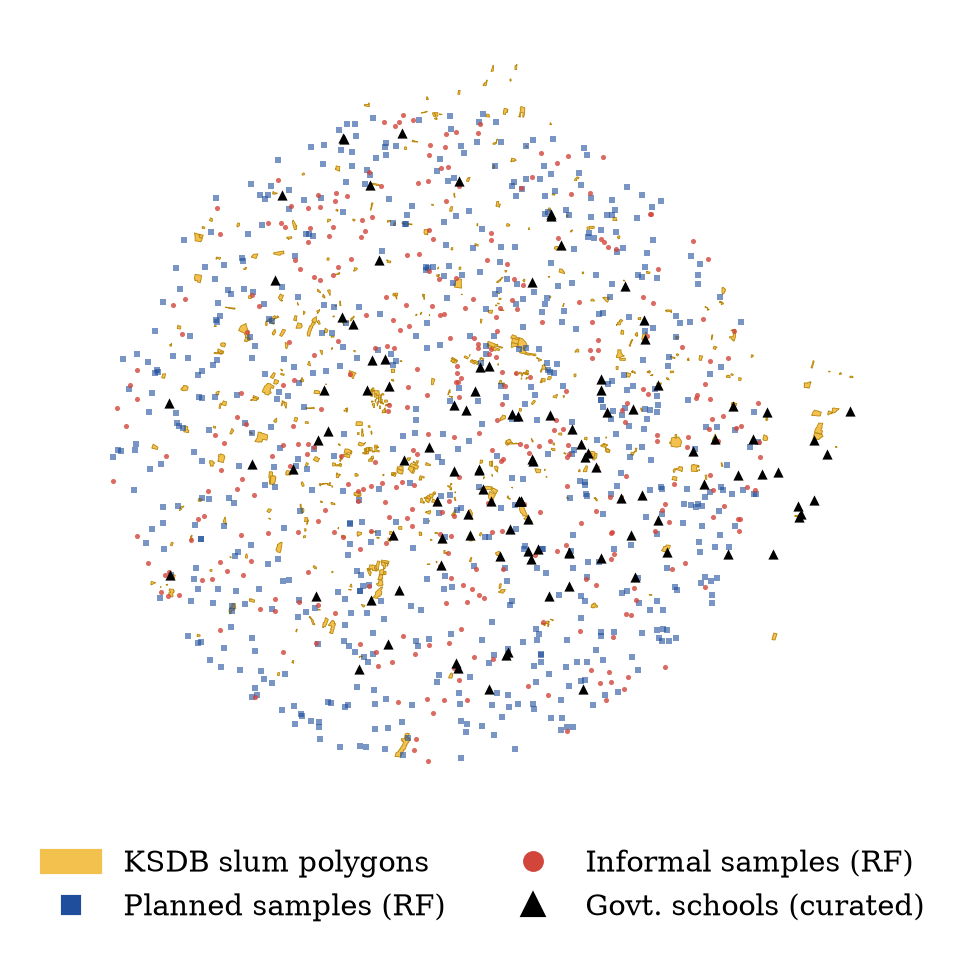
\includegraphics[width=0.92\columnwidth]{fig_study_area.png}
\caption{Study area. KSDB slum polygons (yellow), Random Forest sample locations classified as planned (blue squares) and informal (red circles) within the 15\km{} classification radius, and the 111 curated government schools (black triangles).}
\label{fig:study}
\end{figure}

\subsection{Datasets}
Table~\ref{tab:data} lists the datasets. All are open or publicly released.

\begin{table}[!t]
\centering
\caption{Datasets Used}
\label{tab:data}
\footnotesize
\begin{tabularx}{\columnwidth}{@{}p{1.75cm}Xp{2.2cm}@{}}
\toprule
\textbf{Dataset} & \textbf{Content used} & \textbf{Size} \\
\midrule
Sentinel-2 L2A \cite{drusch2012} & Surface reflectance B4, B8, B11; Jan--Feb 2024 median composite, cloud $<5\%$ & 10\m{} raster \\
OSM walk network \cite{boeing2017} & Pedestrian-accessible ways, private access excluded & 186,595 nodes; 499,950 directed edges \\
OSM schools & \texttt{amenity=school} features with names & 1,464 features \\
KSDB slums & Slum polygons with zone and notification status & 509 polygons \\
WorldPop 2020 \cite{tatem2017} & 100\m{} population, summed per slum polygon & 226,753 residents \\
\bottomrule
\end{tabularx}
\end{table}

\subsection{School Data and the Government-School Definition}
OSM returned 1,464 school features (886 building or campus polygons and 578 points), of which 202 are unnamed. OSM ownership tags are sparse in Bengaluru, so government schools must be identified largely from names. The initial pipeline used a \emph{broad} filter: \texttt{operator:type} matching ``public'' or ``government'', or a name containing ``Govt'', ``Government'', ``BBMP'' or ``Public''. It selected 271 schools. Inspection showed that 150 of these carry no government keyword, and 125 matched only on ``Public''. In Indian usage this word is common in private school names, and several of the schools in the broad set are visibly private institutions.

We therefore define a \emph{curated} set of government schools. A school is included only if a government keyword (government, govt, BBMP, GHPS, GLPS, GHS, GULPS, KGBV, corporation or municipal) appears in the leading part of its name, i.e., not merely in an address suffix such as ``, BBMP Agara''. Colleges and pre-university institutions are excluded. The curated set contains 111 schools, 49 of which are explicitly named as primary schools. The curated set is used for all primary results; the broad set is reported for comparison with the original pipeline (Table~\ref{tab:schools}).

\begin{table}[!t]
\centering
\caption{Government-School Identification}
\label{tab:schools}
\footnotesize
\begin{tabular}{@{}lr@{}}
\toprule
\textbf{Stage} & \textbf{Count} \\
\midrule
All OSM \texttt{amenity=school} features & 1,464 \\
Broad filter (initial pipeline) & 271 \\
\quad of which matched only on ``Public'' & 125 \\
\quad of which carry any government keyword & 121 \\
\quad keyword only in address suffix (removed) & 3 \\
\quad colleges / pre-university (removed) & 7 \\
\textbf{Curated government schools} & \textbf{111} \\
\quad explicitly primary-named & 49 \\
Non-government schools (all others) & 1,353 \\
\bottomrule
\end{tabular}
\end{table}

\begin{figure}[!t]
\centering
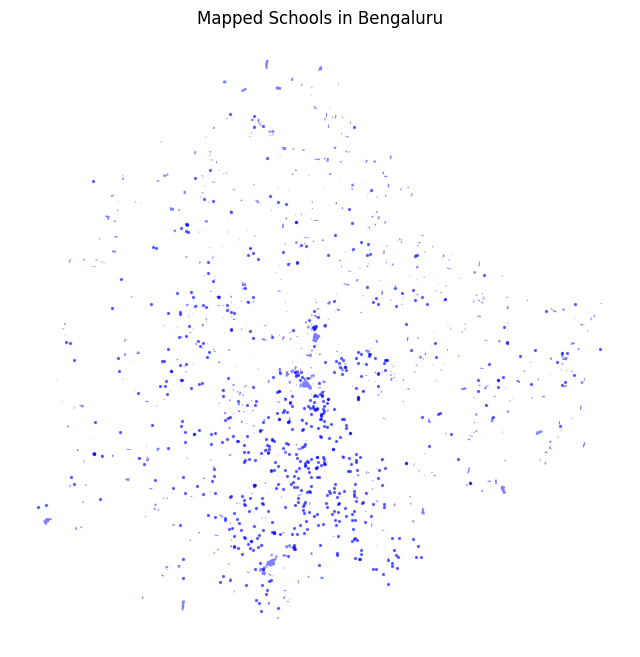
\includegraphics[width=0.85\columnwidth]{mapped_all_schools_bengaluru.png}
\caption{All 1,464 OSM school features in Bengaluru (points and campus polygons).}
\label{fig:allschools}
\end{figure}

\begin{figure}[!t]
\centering
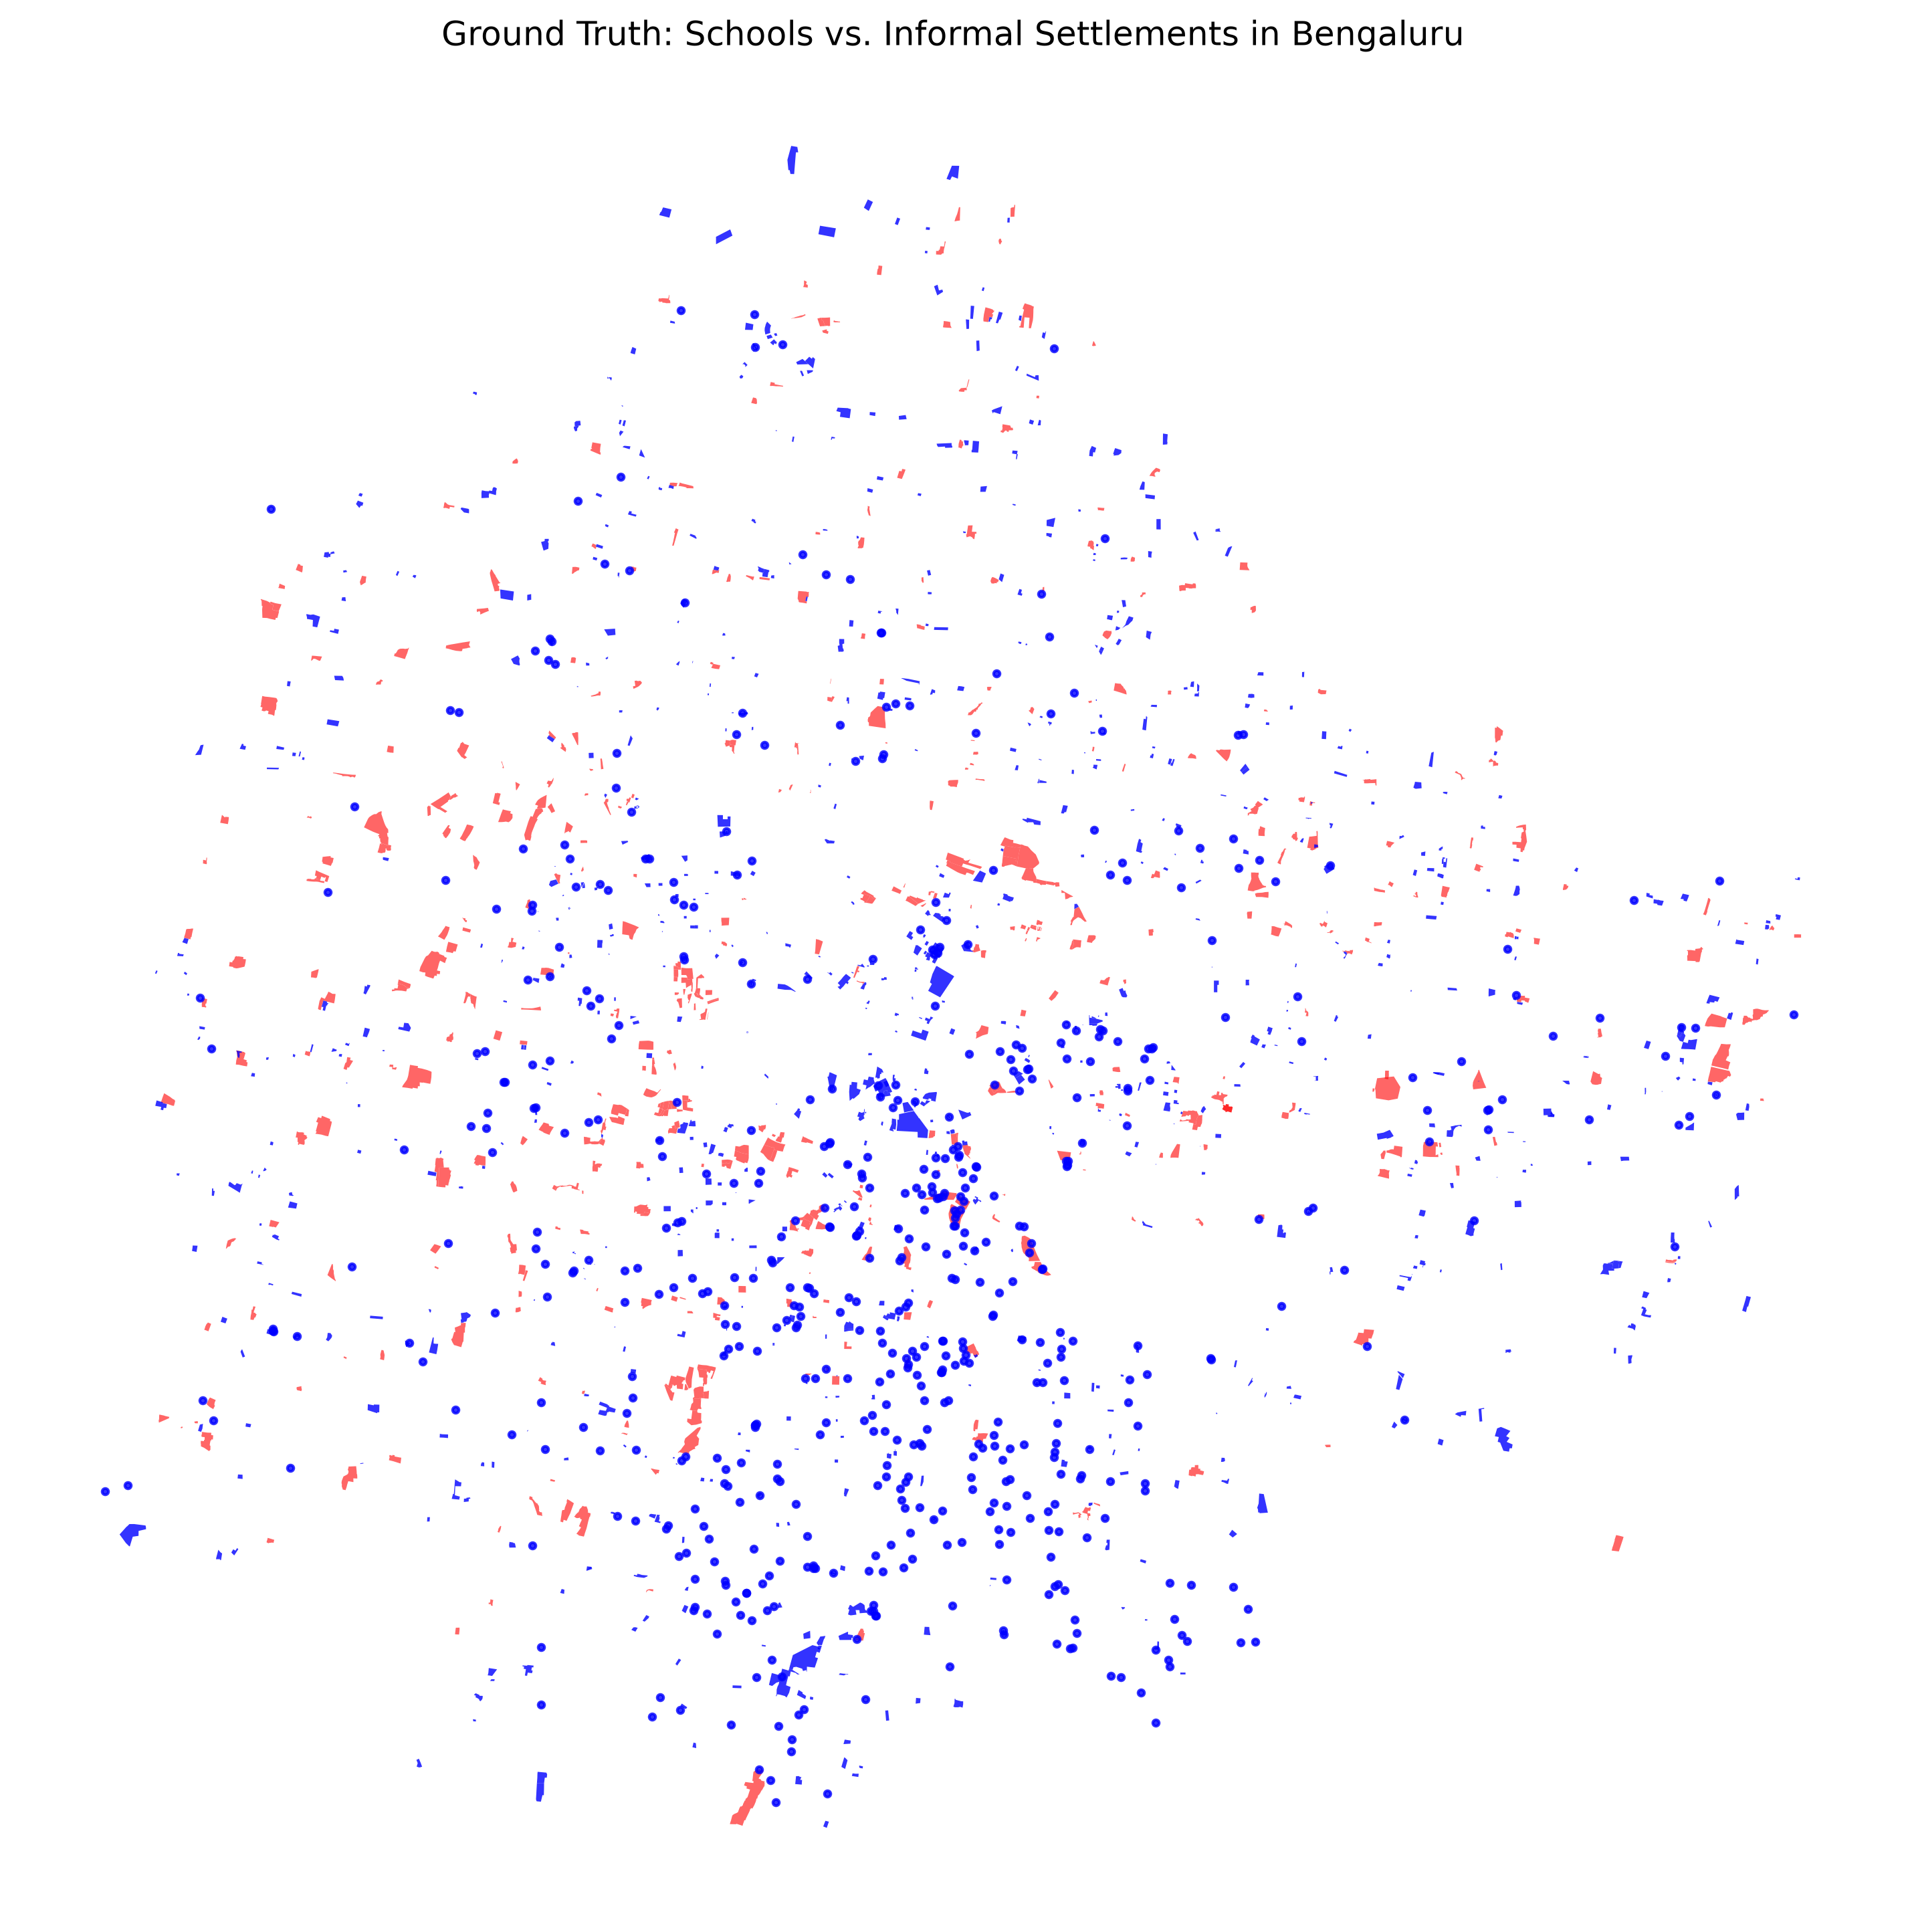
\includegraphics[width=0.92\columnwidth]{ground_truth_schools.png}
\caption{Ground truth overlay: all OSM schools (blue) and KSDB informal-settlement polygons (red).}
\label{fig:gt}
\end{figure}

\begin{figure}[!t]
\centering
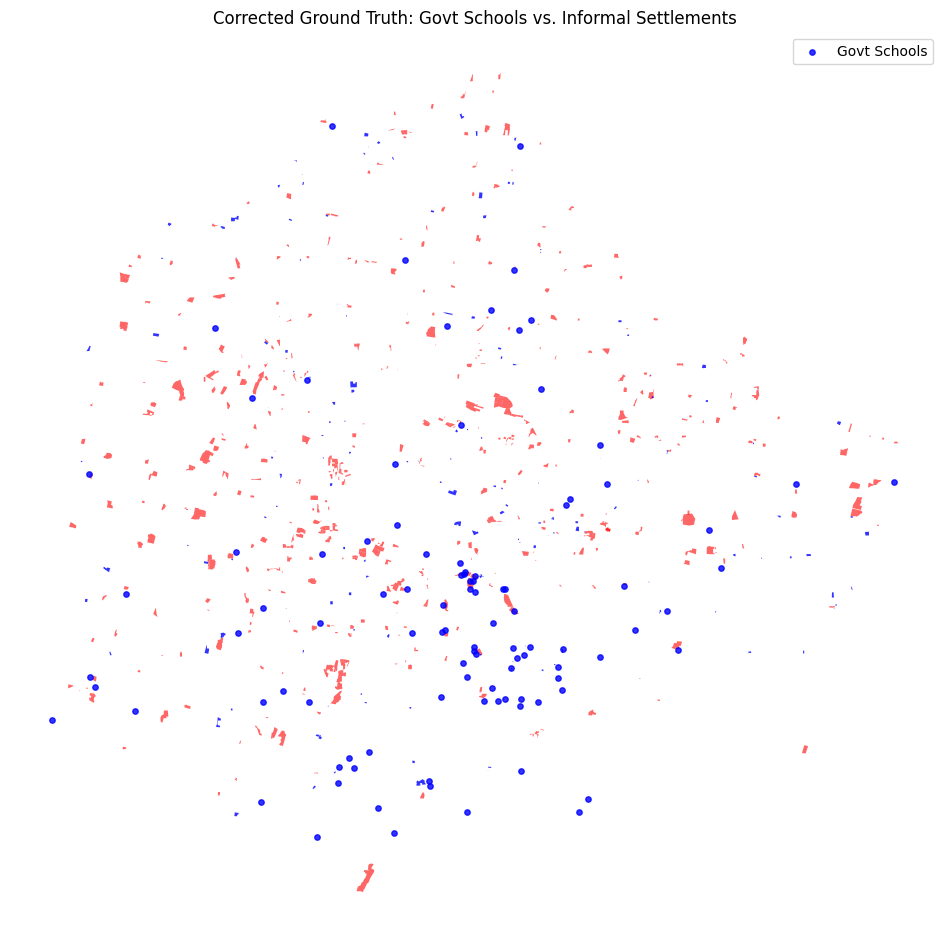
\includegraphics[width=0.92\columnwidth]{govt_schools_vs_informal_settlements.png}
\caption{Government schools selected by the broad filter of the initial pipeline (blue points) and KSDB informal-settlement polygons (red). The curated set used for the primary results is a subset of these schools.}
\label{fig:govtgt}
\end{figure}

%=====================================================================
\section{Proposed Methodology}\label{sec:method}
%=====================================================================
Fig.~\ref{fig:pipeline} shows the four-phase pipeline. The phases are described below.

\begin{figure*}[!t]
\centering
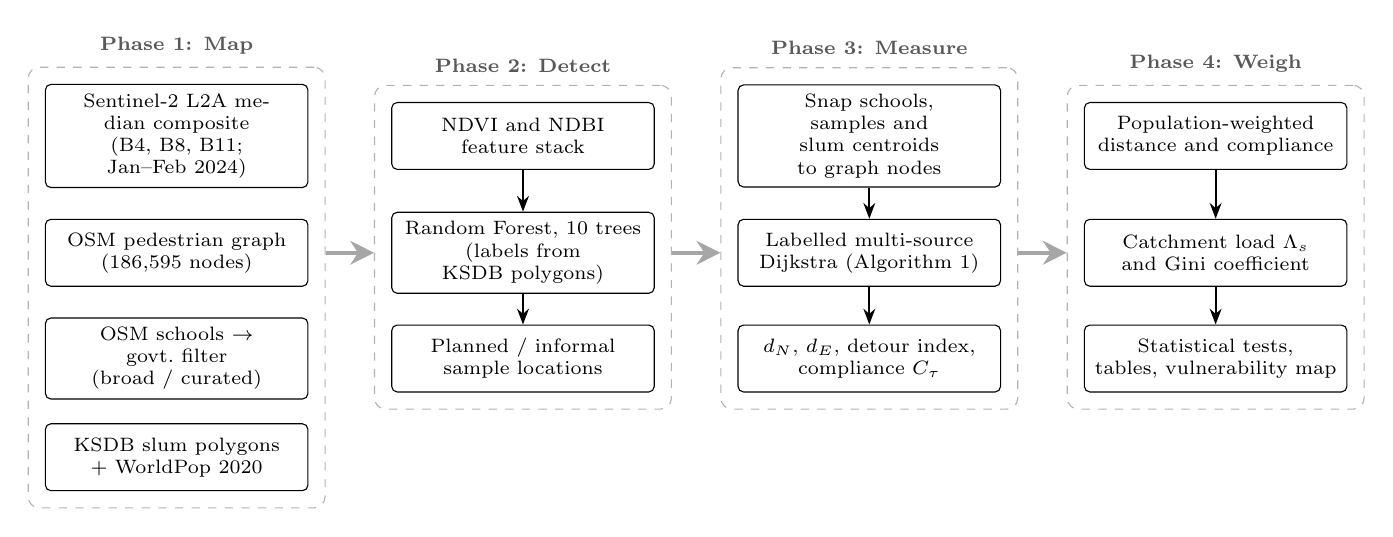
\begin{tikzpicture}[
  box/.style={draw, rounded corners=2pt, align=center, font=\scriptsize, minimum height=0.85cm, text width=3.1cm, fill=white},
  phase/.style={draw=gray!60, dashed, rounded corners=4pt, inner sep=6pt},
  lbl/.style={font=\scriptsize\bfseries, text=gray!70!black},
  arr/.style={-{Stealth[length=2mm]}, thick},
  big/.style={-{Stealth[length=3mm,width=3mm]}, line width=1.4pt, gray!70}]
\matrix[row sep=0.3cm, column sep=1.05cm] {
\node[box] (a1) {Sentinel-2 L2A median composite\\(B4, B8, B11; Jan--Feb 2024)}; &
\node[box] (b1) {NDVI and NDBI\\feature stack}; &
\node[box] (c1) {Snap schools, samples and\\slum centroids to graph nodes}; &
\node[box] (d1) {Population-weighted\\distance and compliance}; \\
\node[box] (a2) {OSM pedestrian graph\\(186,595 nodes)}; &
\node[box] (b2) {Random Forest, 10 trees\\(labels from KSDB polygons)}; &
\node[box] (c2) {Labelled multi-source\\Dijkstra (Algorithm 1)}; &
\node[box] (d2) {Catchment load $\Lambda_s$\\and Gini coefficient}; \\
\node[box] (a3) {OSM schools $\rightarrow$\\govt.\ filter (broad / curated)}; &
\node[box] (b3) {Planned / informal\\sample locations}; &
\node[box] (c3) {$d_N$, $d_E$, detour index,\\compliance $C_\tau$}; &
\node[box] (d3) {Statistical tests,\\tables, vulnerability map}; \\
\node[box] (a4) {KSDB slum polygons\\+ WorldPop 2020}; &
& & \\
};
\foreach \c in {b,c,d} {\draw[arr] (\c1) -- (\c2); \draw[arr] (\c2) -- (\c3);}
\node[phase, fit=(a1)(a4)] (p1) {};
\node[phase, fit=(b1)(b3)] (p2) {};
\node[phase, fit=(c1)(c3)] (p3) {};
\node[phase, fit=(d1)(d3)] (p4) {};
\node[lbl, above=1pt of p1] {Phase 1: Map};
\node[lbl, above=1pt of p2] {Phase 2: Detect};
\node[lbl, above=1pt of p3] {Phase 3: Measure};
\node[lbl, above=1pt of p4] {Phase 4: Weigh};
\draw[big] (p1.east |- b2) -- (p2.west |- b2);
\draw[big] (p2.east |- c2) -- (p3.west |- c2);
\draw[big] (p3.east |- d2) -- (p4.west |- d2);
\end{tikzpicture}
\caption{Proposed pipeline. Phase 1 ingests open data; Phase 2 classifies built-up morphology from Sentinel-2 (training labels drawn from KSDB polygons); Phase 3 computes network distances with a labelled multi-source Dijkstra search; Phase 4 weights results by population and derives catchment loads.}
\label{fig:pipeline}
\end{figure*}

\subsection{Phase 1: Data Acquisition and Pre-processing (Map)}
Three ingestion streams initialise the pipeline. (i) A Sentinel-2 surface-reflectance median composite is built in GEE from scenes acquired between 1 January and 1 March 2024 (the dry season) with less than 5\% cloudy pixels, clipped to the 15\km{} study radius. The median operator suppresses transient clouds and shadows. (ii) The pedestrian network is downloaded with OSMnx using \texttt{network\_type="walk"} and a custom filter that excludes area features and ways tagged \texttt{access=private}. The graph has 186,595 nodes and 499,950 directed edges, with a median edge length of 40.4\m{} (mean 61.0\m{}). (iii) School features are fetched with \texttt{features\_from\_place} for \texttt{amenity=school}. Polygon features are reduced to centroids computed in the projected UTM zone 43N coordinate system (EPSG:32643) and then converted back to WGS-84.

\subsection{Phase 2: Satellite Classification of Built-up Morphology (Detect)}
Two spectral indices are computed from the composite:
\begin{equation}
\mathrm{NDVI}=\frac{\rho_{\mathrm{NIR}}-\rho_{\mathrm{Red}}}{\rho_{\mathrm{NIR}}+\rho_{\mathrm{Red}}}=\frac{B8-B4}{B8+B4},
\end{equation}
\begin{equation}
\mathrm{NDBI}=\frac{\rho_{\mathrm{SWIR}}-\rho_{\mathrm{NIR}}}{\rho_{\mathrm{SWIR}}+\rho_{\mathrm{NIR}}}=\frac{B11-B8}{B11+B8}.
\end{equation}
NDVI \cite{tucker1979} suppresses vegetated pixels such as parks and tree-lined avenues; NDBI \cite{zha2003} emphasises impervious surfaces. The feature vector for each pixel is $\mathbf{x}=[B4, B8, B11, \mathrm{NDVI}, \mathrm{NDBI}]$.

Training data are drawn at 10\m{} scale. Class~1 (informal) consists of 2,000 pixels sampled inside KSDB slum polygons. Class~0 (planned) consists of 2,000 built-up pixels ($\mathrm{NDBI}>0$) sampled outside all slum polygons. A Random Forest \cite{breiman2001} with 10 trees is trained in GEE and applied to the full study area. Sample locations (``virtual students'') are then drawn at random from each predicted class; the exported sample files contain 364 informal and 636 planned locations. Table~\ref{tab:rf} lists the configuration.

\begin{table}[!t]
\centering
\caption{Classification Configuration}
\label{tab:rf}
\footnotesize
\begin{tabular}{@{}ll@{}}
\toprule
\textbf{Parameter} & \textbf{Value} \\
\midrule
Imagery & Sentinel-2 SR (harmonised), median composite \\
Acquisition window & 1 Jan -- 1 Mar 2024 \\
Cloud filter & \texttt{CLOUDY\_PIXEL\_PERCENTAGE} $<5$ \\
Study extent & 15\km{} radius around city centre \\
Features & B4, B8, B11, NDVI, NDBI \\
Training pixels & 2,000 informal + 2,000 planned \\
Classifier & Random Forest, 10 trees \\
Sampling scale & 10\m{} \\
Output samples & 364 informal, 636 planned \\
\bottomrule
\end{tabular}
\end{table}

\subsection{Phase 3: Network Accessibility (Measure)}
Let $G=(V,E,w)$ be the directed pedestrian graph with edge weights $w(e)$ equal to segment length in metres. Every origin $p$ (a sample location or slum centroid) and every school $s\in S$ is snapped to its nearest graph node, $v(p)$ and $v(s)$. The network distance from $p$ to the nearest government school is
\begin{equation}
d_N(p)=\min_{s\in S}\; \mathrm{dist}_G\big(v(p),v(s)\big),
\end{equation}
and the corresponding straight-line distance, computed in UTM coordinates, is
\begin{equation}
d_E(p)=\min_{s\in S}\; \lVert \mathbf{u}(p)-\mathbf{u}(s)\rVert_2 .
\end{equation}
Computing $d_N$ by running one shortest-path search per origin would be wasteful. Instead, we run a single multi-source Dijkstra search \cite{dijkstra1959} seeded simultaneously from all school nodes. Propagating the index of the seeding school as a \emph{label} alongside the tentative distance yields, on termination, both the distance to the nearest school and its identity at every node (Algorithm~1). This is the standard construction of the graph (network) Voronoi diagram \cite{erwig2000,okabe2008}; each Voronoi cell is the walking catchment of one school. The search runs in $O\big((|V|+|E|)\log|V|\big)$ time; on the Bengaluru graph a full pass takes a few seconds on a laptop.

\begin{figure}[!t]
\hrule height 0.8pt\vspace{3pt}
\noindent\textbf{Algorithm 1:} Labelled multi-source Dijkstra\vspace{2pt}
\hrule\vspace{3pt}
{\footnotesize
\noindent\textbf{Input:} graph $G=(V,E,w)$; school nodes $s_1,\dots,s_k$\\
\textbf{Output:} distance $D[v]$ and nearest-school label $L[v]$ for all reachable $v$
\begin{enumerate}\setlength\itemsep{0pt}
\item $D[v]\leftarrow\infty$ for all $v\in V$; priority queue $Q\leftarrow\emptyset$
\item \textbf{for} $i=1$ \textbf{to} $k$: \textbf{if} $D[s_i]=\infty$: $D[s_i]\leftarrow0$; $L[s_i]\leftarrow i$; push $(0,s_i,i)$ to $Q$
\item \textbf{while} $Q\neq\emptyset$:
\item \quad pop $(d,u,i)$ with minimum $d$
\item \quad \textbf{if} $d>D[u]$: \textbf{continue} \hfill (stale entry)
\item \quad \textbf{for each} $(u,v)\in E$:
\item \quad\quad \textbf{if} $d+w(u,v)<D[v]$:
\item \quad\quad\quad $D[v]\leftarrow d+w(u,v)$; $L[v]\leftarrow i$; push $(D[v],v,i)$
\item \textbf{return} $D$, $L$
\end{enumerate}}
\vspace{-2pt}\hrule height 0.8pt
\end{figure}

The \emph{detour index} of an origin is $\eta(p)=d_N(p)/d_E(p)$ (with $d_E$ floored at 50\m{} to avoid division by near-zero distances). The RTE compliance rate of a set of origins $P$ at threshold $\tau$ is
\begin{equation}
C_\tau(P)=\frac{1}{|P|}\sum_{p\in P}\mathbf{1}\big[d_N(p)\le\tau\big],
\end{equation}
with $\tau=1{,}000\m{}$ for primary schooling. The crow-flies compliance rate $C^E_\tau$ is defined analogously with $d_E$. The \emph{false-compliance} share is the fraction of crow-flies-compliant origins that are not network-compliant.

\subsection{Phase 4: Population Weighting and Catchment Load (Weigh)}
For each KSDB slum $k$ with WorldPop population $\pi_k$, the population-weighted network distance and population compliance are
\begin{equation}
\bar d_\pi=\frac{\sum_k \pi_k\, d_N(c_k)}{\sum_k \pi_k},\qquad
C^\pi_\tau=\frac{\sum_k \pi_k\,\mathbf{1}[d_N(c_k)\le\tau]}{\sum_k \pi_k},
\end{equation}
where $c_k$ is the slum centroid. Using the labels from Algorithm~1, the \emph{catchment load} of school $s$ is the slum population for which $s$ is the nearest government school by network:
\begin{equation}
\Lambda_s=\sum_k \pi_k\,\mathbf{1}\big[L[v(c_k)]=s\big].
\end{equation}
Inequality of loads across schools is summarised with the Gini coefficient
\begin{equation}
\mathcal{G}=\frac{\sum_{i}\sum_{j}|\Lambda_i-\Lambda_j|}{2|S|^2\,\bar\Lambda}.
\end{equation}
Because school enrolment capacity is not available for Bengaluru in open form, $\Lambda_s$ measures the \emph{potential} demand that falls on each school, not its utilisation.

\subsection{Statistical Analysis}
Network distances are right-skewed, so formal and informal samples are compared with the two-sided Mann--Whitney $U$ test \cite{mann1947}. Effect size is reported as Cliff's $\delta$ \cite{cliff1993}, interpreted with the thresholds of Romano \textit{et al.}\ \cite{romano2006} ($|\delta|<0.147$ negligible, $<0.33$ small, $<0.474$ medium). The full distributions are compared with the two-sample Kolmogorov--Smirnov test. Compliance proportions are compared with a $\chi^2$ test. A 95\% confidence interval for the difference in means is obtained by the percentile bootstrap with 5,000 resamples \cite{efron1993}.

\subsection{Implementation}
Classification runs in GEE through its Python API and \texttt{geemap}. Routing and analysis use Python 3 with OSMnx 2.1, NetworkX, GeoPandas, SciPy, and Matplotlib. Every number and figure in Section~\ref{sec:results} is regenerated by a single script, \texttt{scripts/paper\_analysis.py}, which runs in about 20\,s after the graph is cached.

%=====================================================================
\section{Results}\label{sec:results}
%=====================================================================
\subsection{Walking Distance from Classified Locations}
Table~\ref{tab:desc} summarises the network and straight-line distances from the 1,000 sample locations to the nearest curated government school. Distances are long in both zone types. The median planned location is 2.07\km{} from a government school by network and the median informal location is 1.92\km{}. Only 16.5\% of planned and 18.7\% of informal locations are within the 1\km{} RTE neighbourhood, and roughly half of each group is more than 2\km{} away. Fig.~\ref{fig:mean} compares the means under both school definitions, and Fig.~\ref{fig:ecdf} shows the full cumulative distributions.

\begin{table}[!t]
\centering
\caption{Distance to Nearest Government School (Curated Set, $n=111$ Schools)}
\label{tab:desc}
\footnotesize
\begin{threeparttable}
\begin{tabular}{@{}lrrrr@{}}
\toprule
& \multicolumn{2}{c}{\textbf{Network $d_N$ (m)}} & \multicolumn{2}{c}{\textbf{Straight line $d_E$ (m)}} \\
\cmidrule(lr){2-3}\cmidrule(l){4-5}
\textbf{Statistic} & \textbf{Planned} & \textbf{Informal} & \textbf{Planned} & \textbf{Informal} \\
\midrule
$n$ & 636 & 364 & 636 & 364 \\
Mean & 2,318 & 2,098 & 1,662 & 1,503 \\
Std.\ dev. & 1,557 & 1,164 & 1,041 & 913 \\
Median & 2,070 & 1,919 & 1,448 & 1,316 \\
Q1 -- Q3 & 1,239--3,024 & 1,244--2,884 & 848--2,245 & 813--1,982 \\
90th pct. & 4,207 & 3,677 & 3,231 & 2,764 \\
$\le$ 1\km{} (\%) & 16.5 & 18.7 & 31.8 & 35.2 \\
$>$ 2\km{} (\%) & 52.7 & 48.1 & 31.8 & 24.5 \\
Median detour $\eta$ & 1.35 & 1.35 & --- & --- \\
\bottomrule
\end{tabular}
\begin{tablenotes}\footnotesize
\item Median snapping distance: 37.6\m{} (planned), 47.0\m{} (informal), 28.8\m{} (schools).
\end{tablenotes}
\end{threeparttable}
\end{table}

\begin{figure*}[!t]
\centering
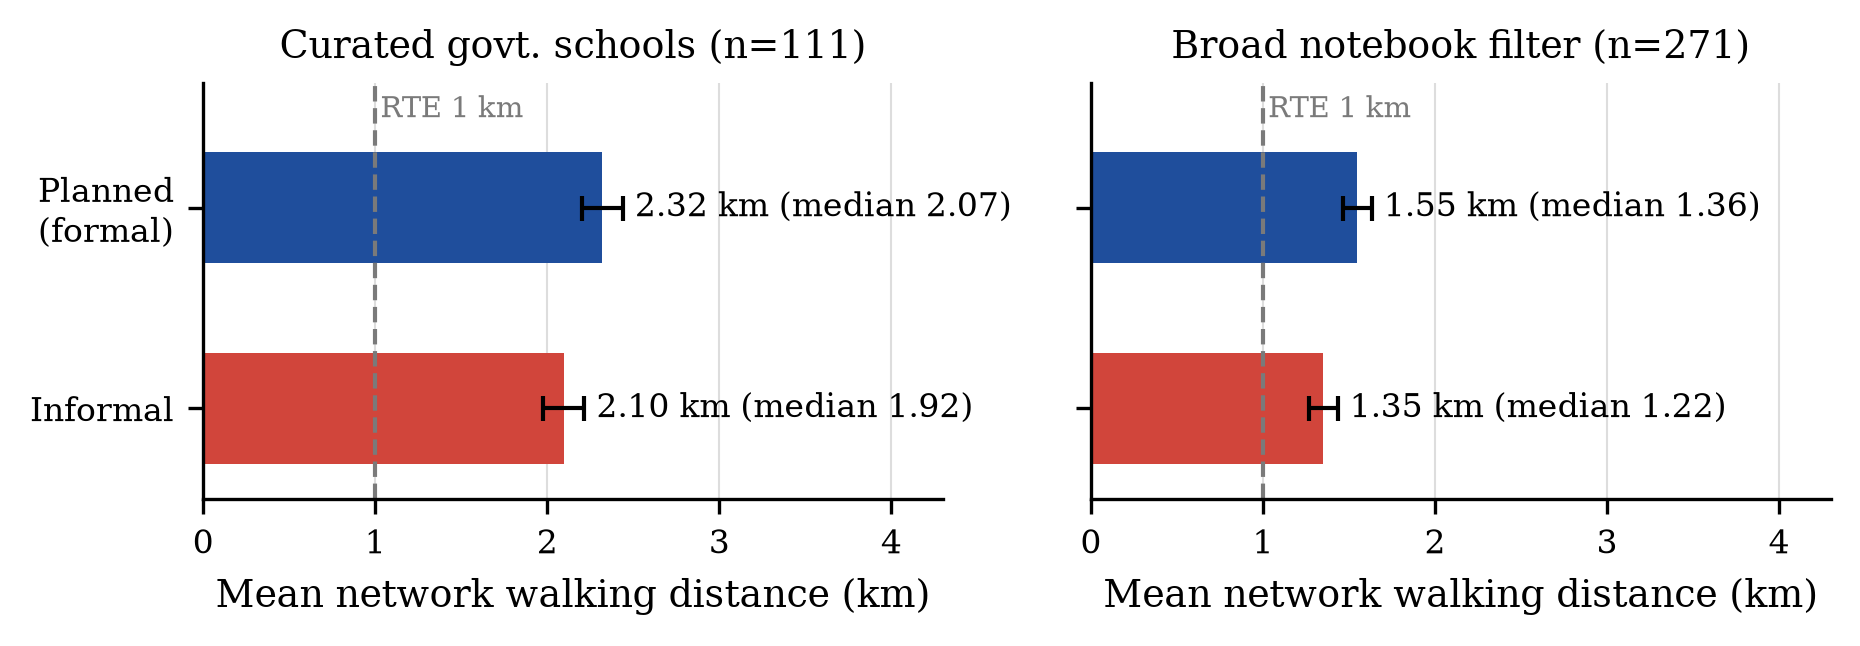
\includegraphics[width=0.78\textwidth]{fig_mean_distance.png}
\caption{Mean network walking distance to the nearest government school, with 95\% bootstrap confidence intervals. Left: curated government schools (primary analysis). Right: broad filter of the initial pipeline, which includes many private ``Public'' schools. The dashed line marks the 1\km{} RTE neighbourhood.}
\label{fig:mean}
\end{figure*}

\begin{figure}[!t]
\centering
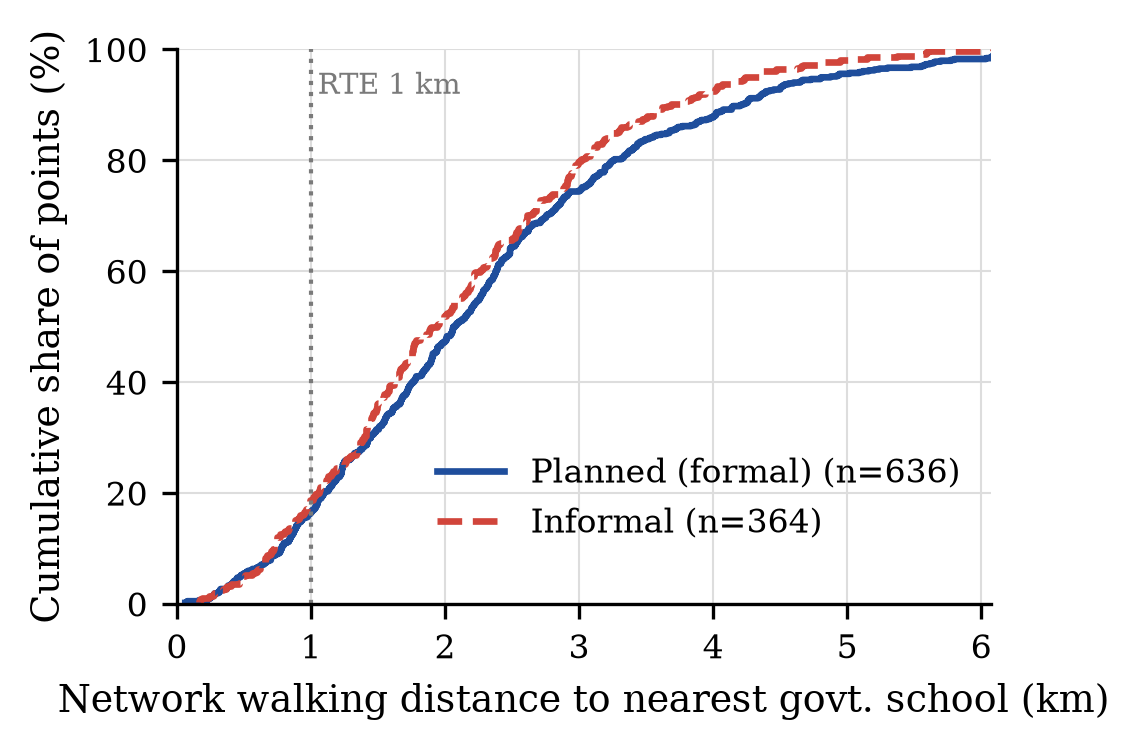
\includegraphics[width=\columnwidth]{fig_distance_ecdf.png}
\caption{Empirical cumulative distribution of network walking distance to the nearest curated government school. The two curves are close throughout; the informal curve lies slightly to the left.}
\label{fig:ecdf}
\end{figure}

\subsection{Formal versus Informal: How Large Is the Difference?}
Table~\ref{tab:tests} reports the statistical comparison. With curated schools, planned locations are on average 220\m{} farther than informal locations (95\% bootstrap CI: 41--382\m{}). However, the rank-based Mann--Whitney test is not significant at the 5\% level ($p=0.094$), the Kolmogorov--Smirnov test finds no difference in distributions ($p=0.18$), the compliance rates do not differ ($\chi^2$ $p=0.43$), and Cliff's $\delta=0.06$ is negligible. With the broad filter, the same direction appears more strongly ($p=0.004$, $\delta=0.11$), but that filter counts private schools as government schools.

The direction of the gap is consistent: planned layouts are, if anything, farther from government schools than informal areas. The magnitude, however, is small compared with the distance both groups must walk. An earlier run of the pipeline on a different OSM snapshot with a 257-school broad filter produced means of 1.60\km{} (planned) and 1.43\km{} (informal), which is consistent with the broad-filter column of Table~\ref{tab:tests}.

\begin{table}[!t]
\centering
\caption{Planned vs.\ Informal Comparison under Two Government-School Definitions}
\label{tab:tests}
\footnotesize
\begin{tabular}{@{}lrr@{}}
\toprule
\textbf{Quantity} & \textbf{Curated (111)} & \textbf{Broad (271)} \\
\midrule
Mean $d_N$, planned (m) & 2,318 & 1,548 \\
Mean $d_N$, informal (m) & 2,098 & 1,351 \\
Mean difference (m) & 220 & 197 \\
95\% bootstrap CI (m) & [41, 382] & [81, 314] \\
Mann--Whitney $U$ & 123,120 & 128,255 \\
\quad $p$-value & 0.094 & 0.004 \\
Cliff's $\delta$ & 0.06 (negl.) & 0.11 (negl.) \\
KS statistic $D$ ($p$) & 0.072 (0.18) & 0.091 (0.04) \\
$\chi^2$ on 1\km{} compliance ($p$) & 0.62 (0.43) & 5.47 (0.02) \\
Compliance $\le$1\km{}, planned (\%) & 16.5 & 32.5 \\
Compliance $\le$1\km{}, informal (\%) & 18.7 & 40.1 \\
\bottomrule
\end{tabular}
\end{table}

\subsection{Sensitivity to the Distance Threshold}
Fig.~\ref{fig:sweep} and Table~\ref{tab:sweep} show compliance as a function of the threshold $\tau$. Compliance rises steeply between 1 and 3\km{}. At 3\km{}, the RTE neighbourhood for upper-primary schooling (Classes VI--VIII), 74.4\% of planned and 79.9\% of informal locations are covered. The shortfall is therefore most severe for the youngest children, for whom the strictest (1\km{}) standard applies.

\begin{figure}[!t]
\centering
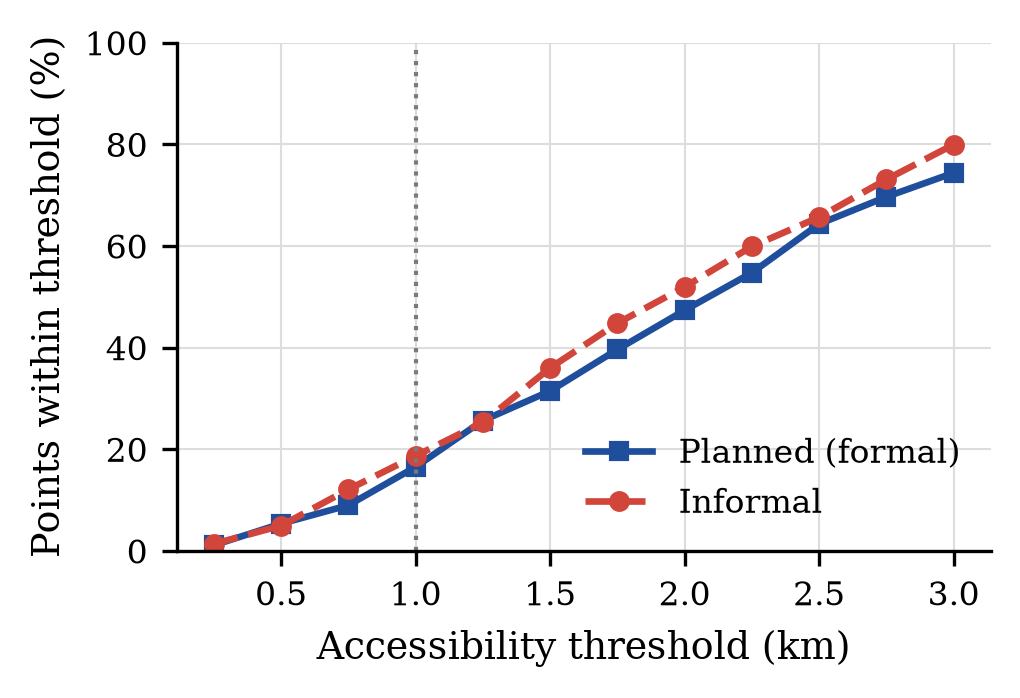
\includegraphics[width=0.9\columnwidth]{fig_threshold_sweep.png}
\caption{Share of sample locations within a given network distance of a curated government school. The dotted line marks the 1\km{} primary-school neighbourhood.}
\label{fig:sweep}
\end{figure}

\begin{table}[!t]
\centering
\caption{Compliance (\%) by Network-Distance Threshold}
\label{tab:sweep}
\footnotesize
\begin{tabular}{@{}lrrrrr@{}}
\toprule
\textbf{Threshold} & \textbf{0.5\km{}} & \textbf{1\km{}} & \textbf{1.5\km{}} & \textbf{2\km{}} & \textbf{3\km{}} \\
\midrule
Planned & 5.3 & 16.5 & 31.4 & 47.3 & 74.4 \\
Informal & 4.9 & 18.7 & 36.0 & 51.9 & 79.9 \\
\bottomrule
\end{tabular}
\end{table}

\subsection{The Crow-Flies Fallacy}\label{sec:crowflies}
Fig.~\ref{fig:euclid} plots network against straight-line distance for every sample location, and Table~\ref{tab:crow} summarises the effect on compliance. Network and Euclidean distances are strongly rank-correlated (Spearman $\rho=0.93$), but the median detour index is 1.35: a typical walk is roughly one-third longer than the straight line. At the 1\km{} threshold this matters a great deal. A straight-line audit would classify 33.0\% of locations as compliant, whereas the network audit finds 17.3\%. Of the locations that a crow-flies buffer would certify as compliant, 48.2\% are actually more than 1\km{} away on foot. With the broad school set the pattern is the same: 58.9\% vs.\ 35.3\%, a false-compliance share of 41.4\%.

\begin{figure}[!t]
\centering
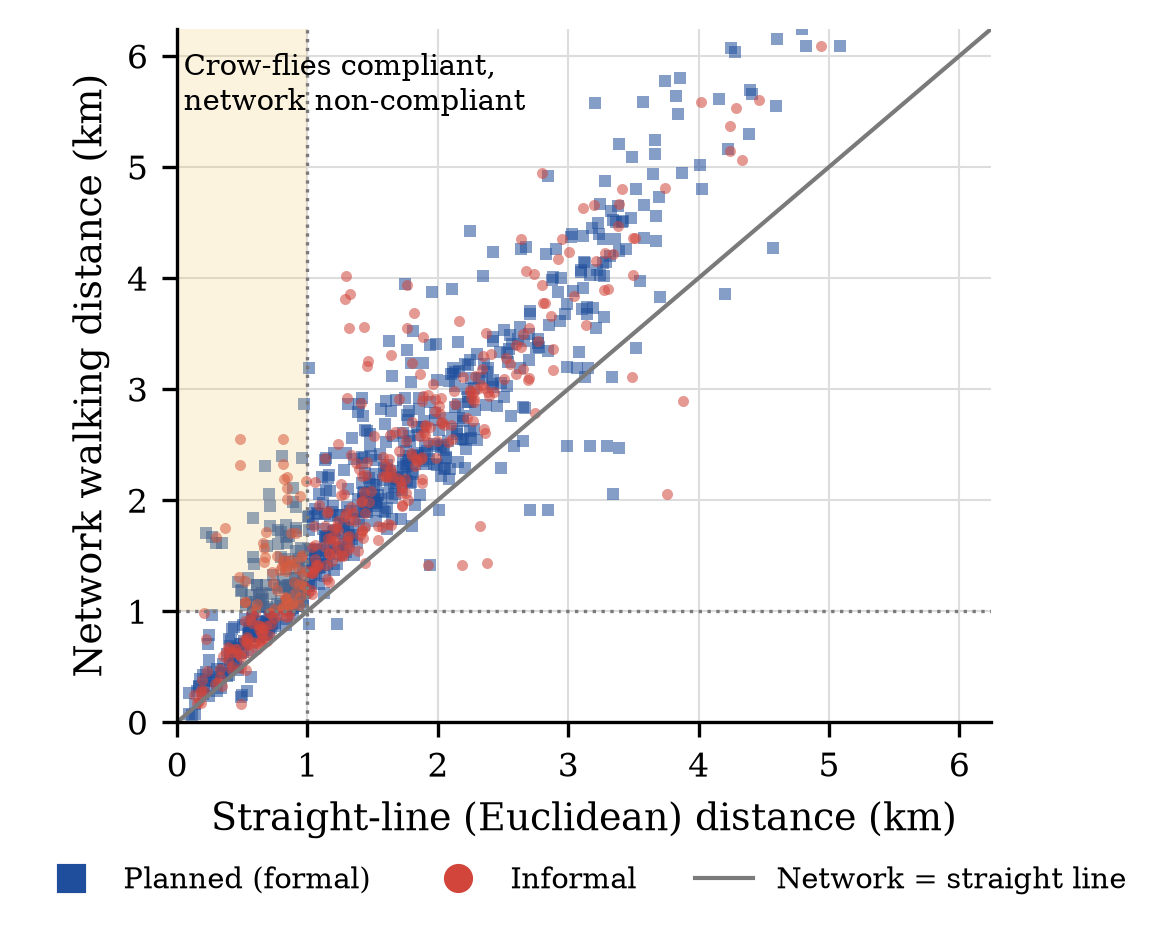
\includegraphics[width=\columnwidth]{fig_euclid_vs_network.png}
\caption{Network vs.\ straight-line distance to the nearest curated government school. Points in the shaded region lie within 1\km{} in a straight line but more than 1\km{} by the street network.}
\label{fig:euclid}
\end{figure}

\begin{table}[!t]
\centering
\caption{Straight-Line vs.\ Network Compliance at 1\km{}}
\label{tab:crow}
\footnotesize
\begin{tabular}{@{}lrr@{}}
\toprule
\textbf{Quantity} & \textbf{Curated} & \textbf{Broad} \\
\midrule
Crow-flies compliant, $C^E_{1\mathrm{km}}$ (\%) & 33.0 & 58.9 \\
Network compliant, $C_{1\mathrm{km}}$ (\%) & 17.3 & 35.3 \\
False-compliant, share of all locations (\%) & 15.9 & 24.4 \\
False-compliant, share of crow-flies compliant (\%) & 48.2 & 41.4 \\
Spearman $\rho(d_N,d_E)$ & 0.93 & 0.87 \\
\bottomrule
\end{tabular}
\end{table}

\subsection{Population-Weighted Access for KSDB Slums}\label{sec:slums}
The classified sample locations depend on the satellite classifier (see Section~\ref{sec:validity}). The KSDB slum polygons offer an independent, register-based view. Table~\ref{tab:slums} reports network access for all 509 polygons, which together hold an estimated 226,753 residents (median slum: 1.25\,ha, 127 residents, 187 residents/ha). With curated schools, the median slum centroid is 1.72\km{} from a government school by network. The population-weighted distance is 2.02\km{}, and only 20.1\% of slum residents live within the 1\km{} RTE neighbourhood. 39.1\% of slums are more than 2\km{} away.

\begin{table}[!t]
\centering
\caption{Network Access for KSDB Slums (WorldPop-Weighted)}
\label{tab:slums}
\footnotesize
\begin{tabular}{@{}lrr@{}}
\toprule
\textbf{Quantity} & \textbf{Curated} & \textbf{Broad} \\
\midrule
Slums routed & 509 & 509 \\
Residents (WorldPop 2020) & 226,753 & 226,753 \\
Median slum distance (m) & 1,723 & 1,103 \\
Population-weighted distance (m) & 2,023 & 1,331 \\
Slums within 1\km{} (\%) & 27.7 & 45.8 \\
Residents within 1\km{} (\%) & 20.1 & 39.2 \\
Slums beyond 2\km{} (\%) & 39.1 & 11.6 \\
Spearman $\rho$(population, distance) & 0.06 ($p$=0.15) & 0.05 ($p$=0.28) \\
\bottomrule
\end{tabular}
\end{table}

Fig.~\ref{fig:slumpop} plots each slum's distance against its population. There is no relationship between settlement size and distance ($\rho=0.06$, $p=0.15$), nor between density and distance ($\rho=-0.02$, $p=0.59$). Large slums are no better served than small ones.

\begin{figure}[!t]
\centering
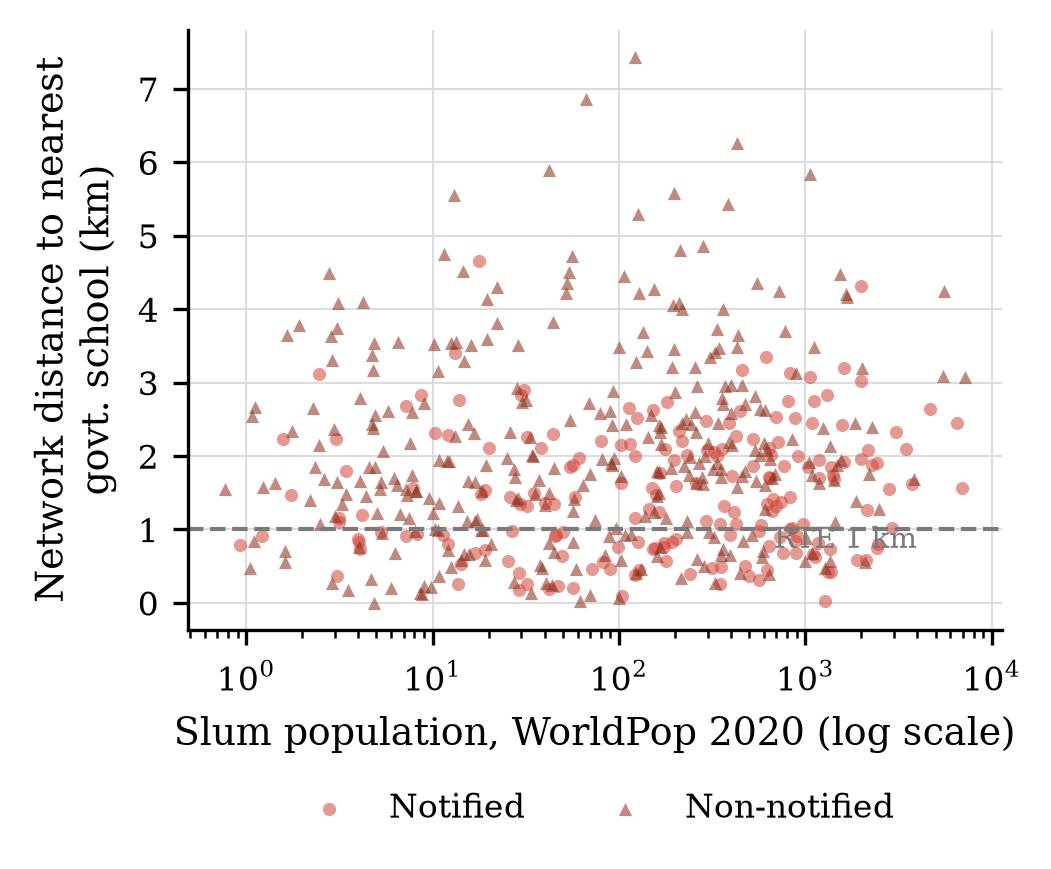
\includegraphics[width=\columnwidth]{fig_slum_pop_vs_distance.png}
\caption{Network distance to the nearest curated government school vs.\ WorldPop population for each KSDB slum, by notification status. Settlement size does not predict proximity.}
\label{fig:slumpop}
\end{figure}

\subsubsection{Notified versus non-notified slums}
Table~\ref{tab:notif} separates slums by notification status. Non-notified slums, i.e., settlements on the register but without legal notification, are significantly farther from government schools than notified ones. The population-weighted distance is 2.40 vs.\ 1.71\km{}, and only 15.5\% of non-notified residents are within 1\km{}, compared with 24.0\% of notified residents (Mann--Whitney $p=1.5\times10^{-6}$, Cliff's $\delta=0.25$, small). The difference persists with the broad school set ($p=0.002$, $\delta=0.16$).

\begin{table}[!t]
\centering
\caption{Access by Slum Notification Status (Curated Schools)}
\label{tab:notif}
\footnotesize
\begin{tabular}{@{}lrr@{}}
\toprule
\textbf{Quantity} & \textbf{Notified} & \textbf{Non-notified} \\
\midrule
Slums & 192 & 317 \\
Residents & 122,705 & 104,049 \\
Median distance (m) & 1,441 & 1,862 \\
Population-weighted distance (m) & 1,707 & 2,396 \\
Slums within 1\km{} (\%) & 35.9 & 22.7 \\
Residents within 1\km{} (\%) & 24.0 & 15.5 \\
\bottomrule
\end{tabular}
\end{table}

\subsubsection{Administrative zones}
Access varies sharply between the city's administrative zones (Table~\ref{tab:zones}, Figs.~\ref{fig:zones} and~\ref{fig:zonebox}). South zone is best served: 43.8\% of its slum residents are within 1\km{}, at a population-weighted distance of 1.17\km{}. Dasarahalli, Yelahanka and Bommanahalli are the worst: population-weighted distances exceed 3\km{}, and in Dasarahalli fewer than 1\% of slum residents are within 1\km{} of a curated government school. The peripheral zones, where much post-2011 growth has occurred, are the least served. The spread within zones is also wide (Fig.~\ref{fig:zonebox}): even in the best-served South zone, a quarter of slums are more than 1.7\km{} from a government school, while in Dasarahalli the median slum is 3.4\km{} away.

\begin{table}[!t]
\centering
\caption{Slum Access by Administrative Zone (Curated Schools)}
\label{tab:zones}
\footnotesize
\begin{tabular}{@{}lrrrr@{}}
\toprule
\textbf{Zone} & \textbf{Slums} & \textbf{Residents} & \textbf{Pop.-wtd.} & \textbf{Res.\ $\le$1\km{}} \\
 & & & \textbf{dist.\ (m)} & \textbf{(\%)} \\
\midrule
South & 93 & 48,486 & 1,167 & 43.8 \\
Mahadevapura & 90 & 1,366 & 1,507 & 35.8 \\
West & 90 & 67,150 & 1,889 & 17.9 \\
East & 103 & 54,730 & 2,079 & 17.6 \\
RR Nagar & 55 & 24,690 & 2,443 & 4.4 \\
Yelahanka & 46 & 11,101 & 3,170 & 8.6 \\
Bommanahalli & 14 & 325 & 3,174 & 10.1 \\
Dasarahalli & 18 & 18,906 & 3,330 & 0.7 \\
\bottomrule
\end{tabular}
\end{table}

\begin{figure}[!t]
\centering
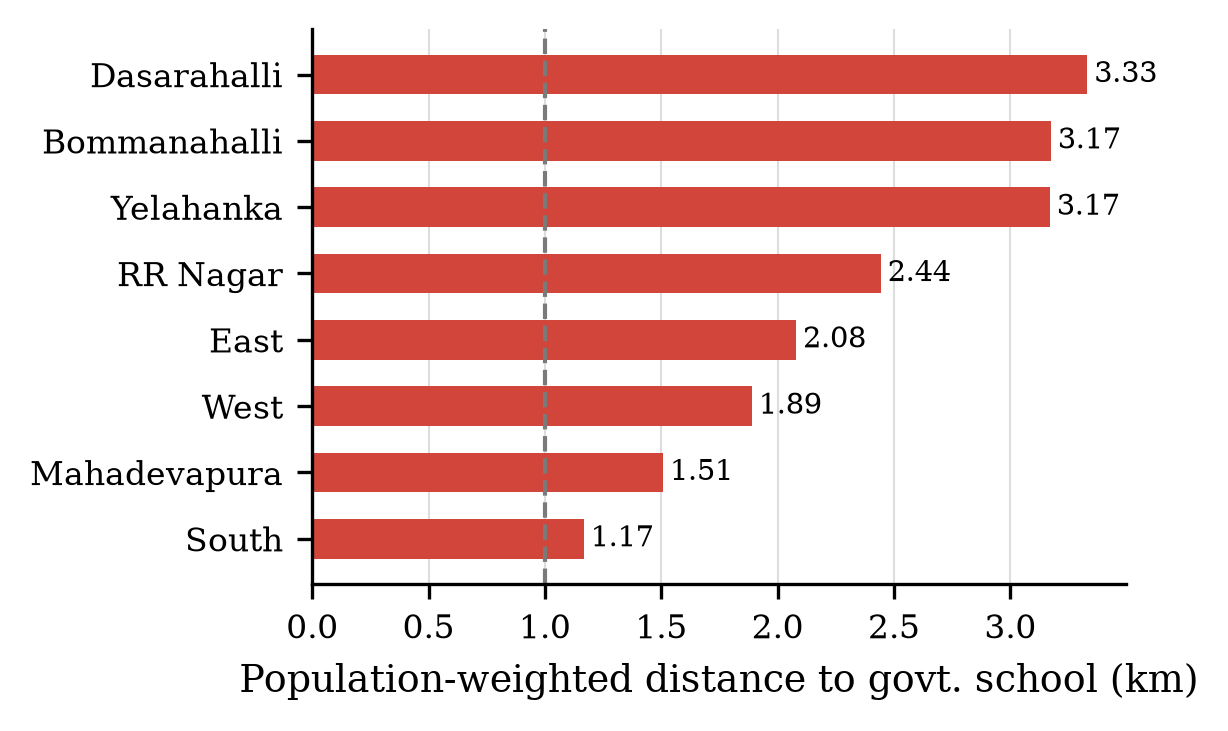
\includegraphics[width=\columnwidth]{fig_zone_distance.png}
\caption{Population-weighted network distance from KSDB slums to the nearest curated government school, by administrative zone.}
\label{fig:zones}
\end{figure}

\begin{figure}[!t]
\centering
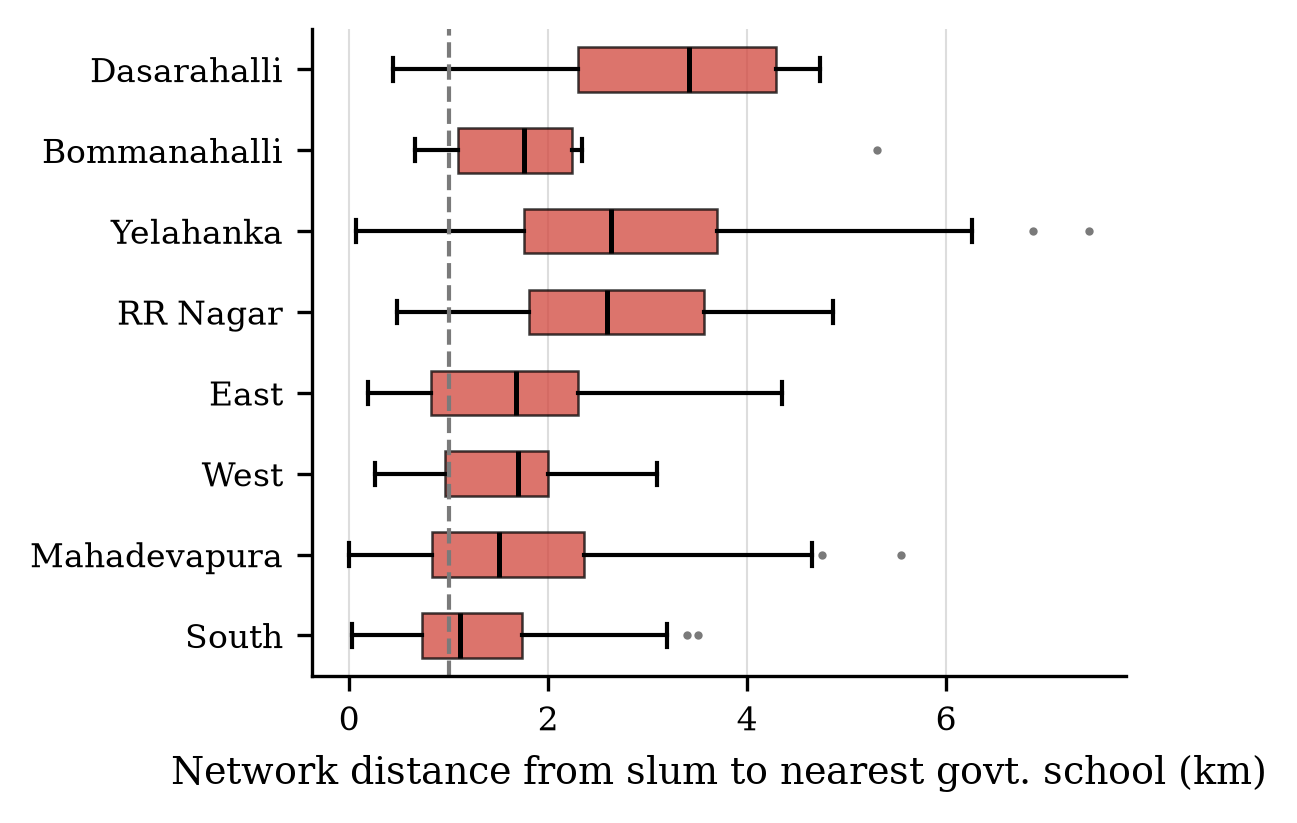
\includegraphics[width=\columnwidth]{fig_zone_boxplot.png}
\caption{Distribution of network distance from each KSDB slum to the nearest curated government school, by administrative zone (boxes: interquartile range; line: median; dashed line: 1\km{} RTE neighbourhood).}
\label{fig:zonebox}
\end{figure}

\subsection{Catchment Load: Where Slum Demand Falls}
Algorithm~1 assigns every slum to its nearest government school. Of the 111 curated schools, 81 are the nearest school for at least one slum, and 30 serve none. The distribution of potential demand is extremely unequal (Fig.~\ref{fig:load}, Table~\ref{tab:load}). The median school with a slum catchment receives 179 slum residents, the mean is 2,799, and the most-loaded school receives 28,193. The ten most-loaded schools are the nearest government option for 71.5\% of all slum residents, and the Gini coefficient of loads is 0.85. With the broad filter the Gini is similar (0.87), but the most-loaded ``government'' schools are private institutions with ``Public'' in their names. This illustrates how misclassification can shift apparent demand onto schools that do not provide free education.

\begin{figure}[!t]
\centering
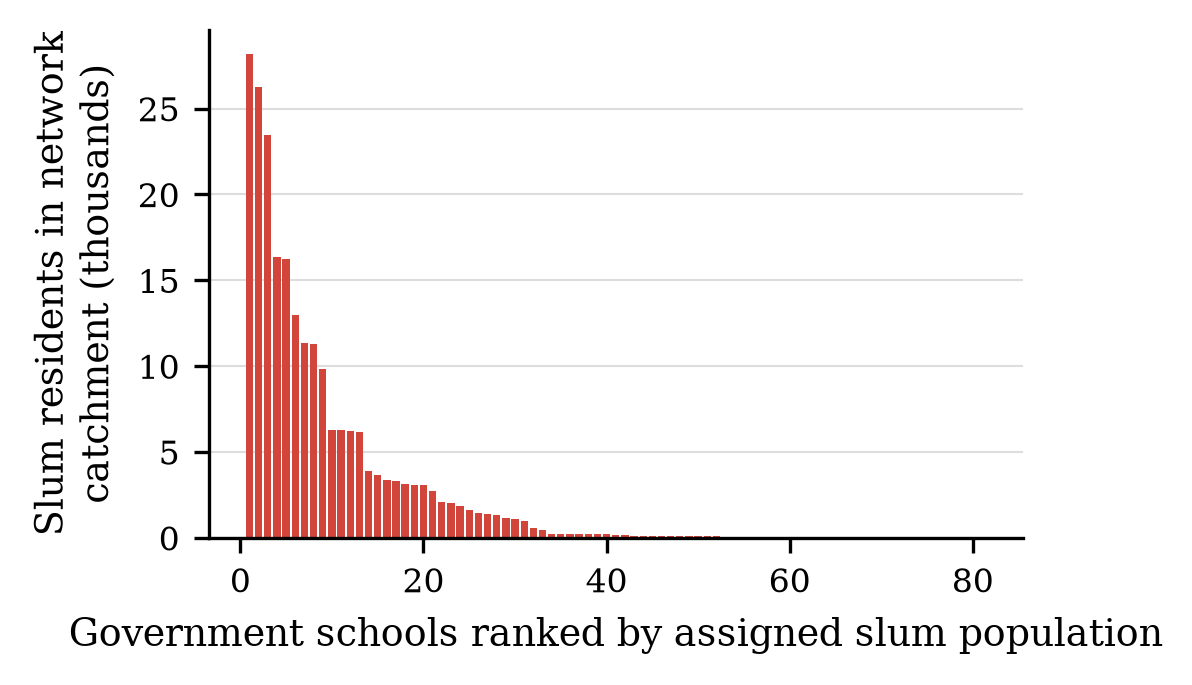
\includegraphics[width=\columnwidth]{fig_catchment_load.png}
\caption{Slum residents for whom each curated government school is the nearest by network, ranked. A small number of schools absorb most potential slum demand.}
\label{fig:load}
\end{figure}

\begin{table}[!t]
\centering
\caption{Most-Loaded Government Schools (Curated Set)}
\label{tab:load}
\footnotesize
\begin{tabularx}{\columnwidth}{@{}Xrr@{}}
\toprule
\textbf{School (OSM name)} & \textbf{Slums} & \textbf{Residents} \\
\midrule
Haji Sir Ismail Sait Govt.\ Urdu \& English HPS & 25 & 28,193 \\
Nammura Government Model Primary School & 22 & 26,242 \\
Government School (generic OSM name) & 27 & 23,453 \\
Gangamma Thimmaiah Govt.\ School & 14 & 16,339 \\
Jindal Government School & 10 & 16,223 \\
\midrule
Top-10 share of slum residents & \multicolumn{2}{r}{71.5\%} \\
Gini coefficient of loads & \multicolumn{2}{r}{0.85} \\
\bottomrule
\end{tabularx}
\end{table}

\subsection{Proximity to Non-Government Schools}
The 1,353 OSM school features outside the curated government set are much closer to every location (Table~\ref{tab:private}). The median planned location is 0.69\km{} from a non-government school and the median informal location 0.60\km{}; 71.2\% and 76.4\% respectively are within 1\km{}. The open data therefore describe a city in which a school of \emph{some} kind is usually within walking distance, but a free government school usually is not.

\begin{table}[!t]
\centering
\caption{Network Distance to Nearest Government vs.\ Non-Government School}
\label{tab:private}
\footnotesize
\begin{tabular}{@{}lrrrr@{}}
\toprule
& \multicolumn{2}{c}{\textbf{Govt.\ (curated)}} & \multicolumn{2}{c}{\textbf{Non-govt.}} \\
\cmidrule(lr){2-3}\cmidrule(l){4-5}
& \textbf{Plan.} & \textbf{Inf.} & \textbf{Plan.} & \textbf{Inf.} \\
\midrule
Median (m) & 2,070 & 1,919 & 691 & 598 \\
Mean (m) & 2,318 & 2,098 & 858 & 757 \\
$\le$ 1\km{} (\%) & 16.5 & 18.7 & 71.2 & 76.4 \\
$>$ 2\km{} (\%) & 52.7 & 48.1 & 5.3 & 4.7 \\
\bottomrule
\end{tabular}
\end{table}

\subsection{Vulnerability and Catchment Maps}
Fig.~\ref{fig:vmapc} maps compliance across the city using the curated government schools: (a) the classified sample locations and (b) the KSDB slums, each coloured by network walking distance. Non-compliant locations dominate the periphery, and the large slums in the West and RR~Nagar zones form the most extensive cluster beyond 2\km{}.

\begin{figure*}[!t]
\centering
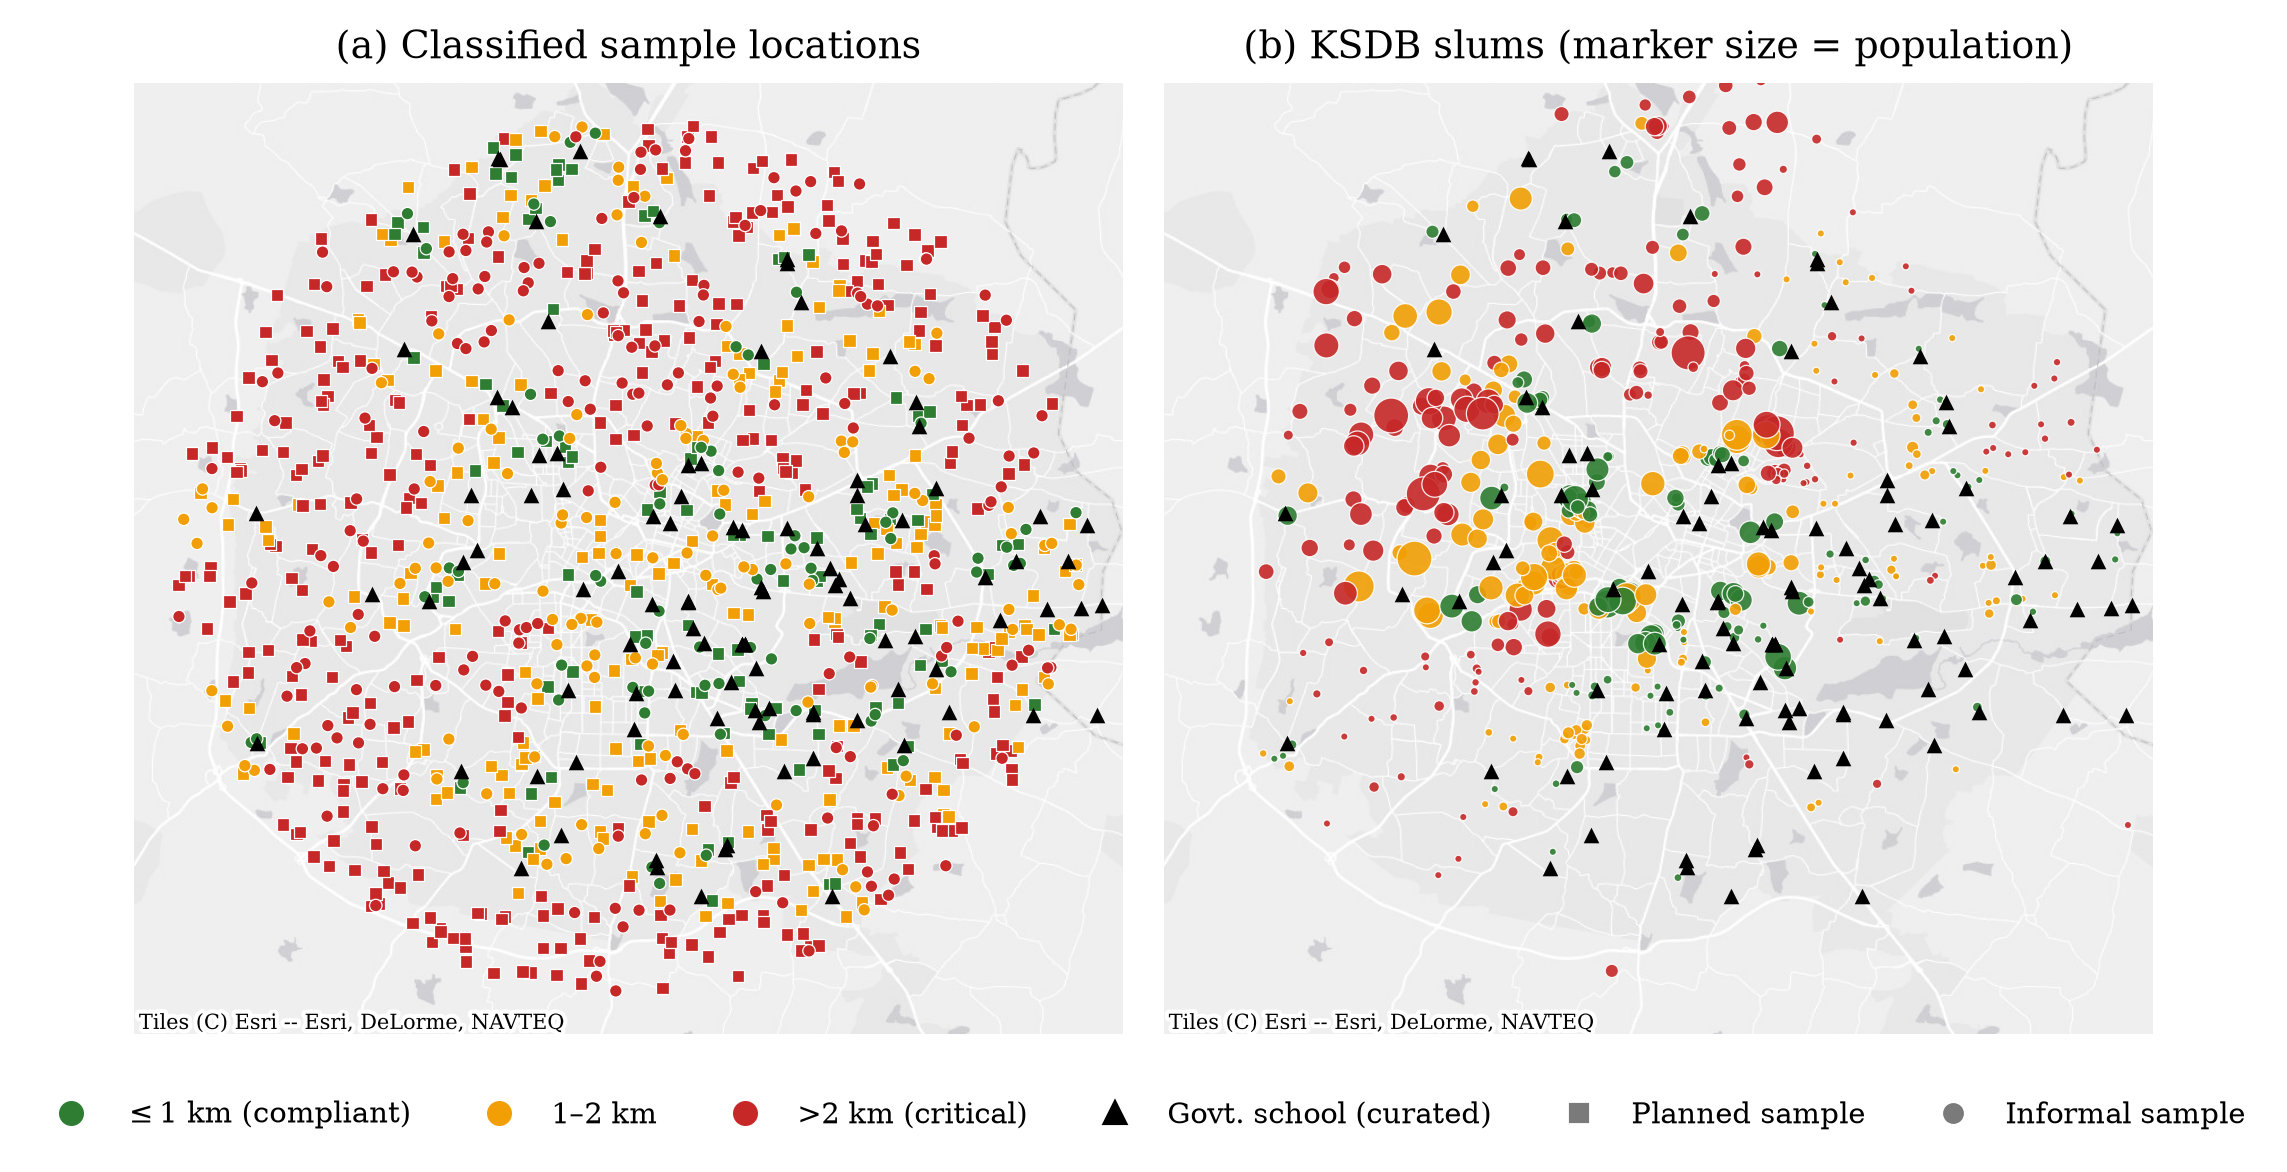
\includegraphics[width=\textwidth]{fig_vulnerability_map.png}
\caption{Vulnerability map of Bengaluru (curated government schools). Colour gives network walking distance to the nearest government school: green $\le$1\km{} (compliant), orange 1--2\km{}, red $>$2\km{} (critical). (a) Random Forest sample locations (squares: planned; circles: informal). (b) KSDB slum centroids, sized by WorldPop population. Black triangles are curated government schools.}
\label{fig:vmapc}
\end{figure*}

Fig.~\ref{fig:catchmap} visualises the network Voronoi partition produced by Algorithm~1. Every street node is coloured by the government school it is nearest to, and nodes more than 1\km{} from any government school are faded. The RTE-compliant area appears as isolated islands around each school rather than a continuous surface, and large parts of the western and northern city---where the biggest slums are concentrated---lie outside every island.

\begin{figure*}[!t]
\centering
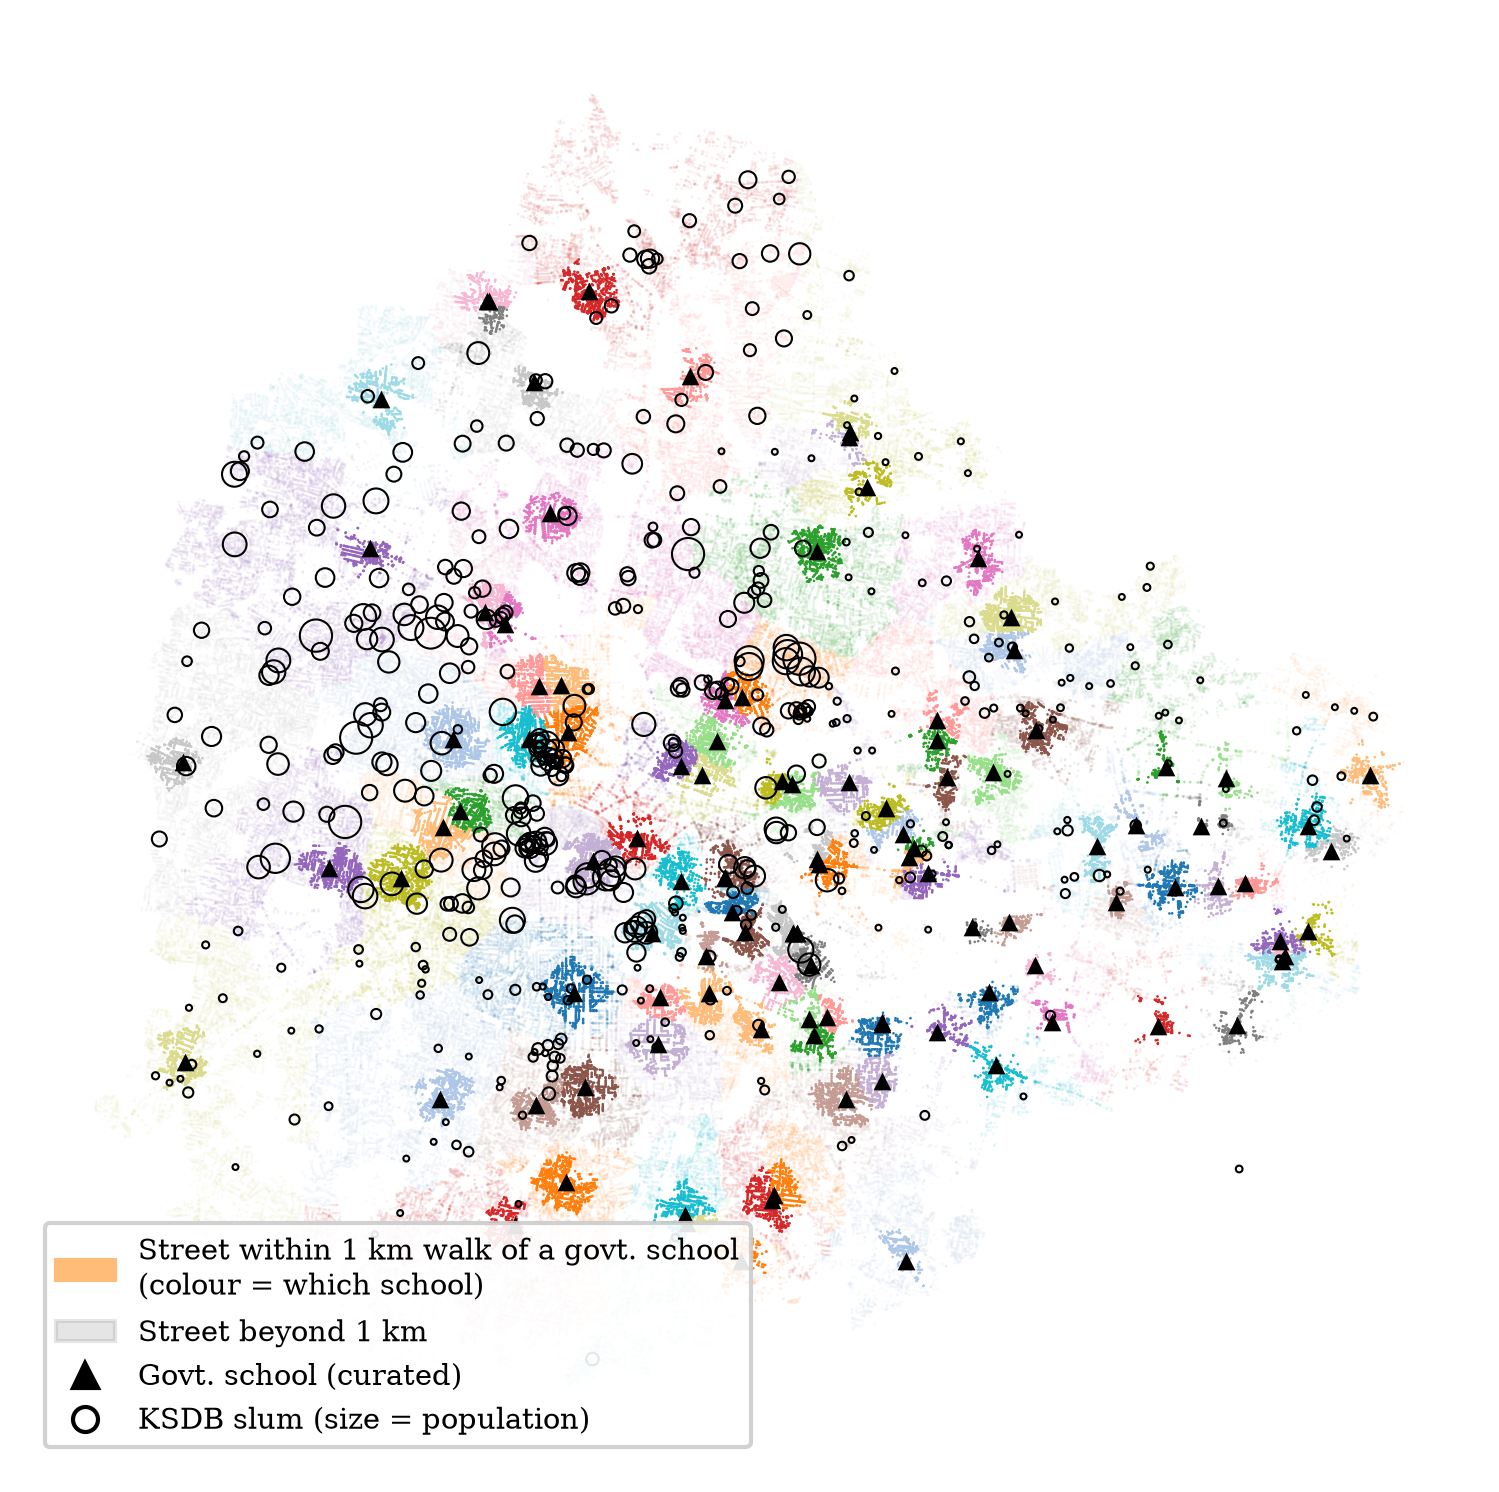
\includegraphics[width=0.82\textwidth]{fig_catchment_map.png}
\caption{Network Voronoi catchments of the 111 curated government schools on the Bengaluru pedestrian network. Each street node is coloured by its nearest government school (colours repeat and only distinguish neighbouring catchments); nodes beyond a 1\km{} walk are faded. Open circles are KSDB slums sized by population; black triangles are schools.}
\label{fig:catchmap}
\end{figure*}

\subsection{Interactive Web Map}
The pipeline also produces an interactive web map (Leaflet via \texttt{folium}) in which every sample location is coloured by its walking distance: green ($\le1\km{}$, compliant), orange (1--2\km{}) and red ($>2\km{}$, critical). Each marker's pop-up reports its zone type and distance, and government schools are shown as small blue points. Figs.~\ref{fig:vmap} and~\ref{fig:vmap2} show two views of the interface. These screenshots come from the initial pipeline and therefore use the broad school filter; an equivalent map built on the curated set is exported alongside the analysis.

\begin{figure*}[!t]
\centering
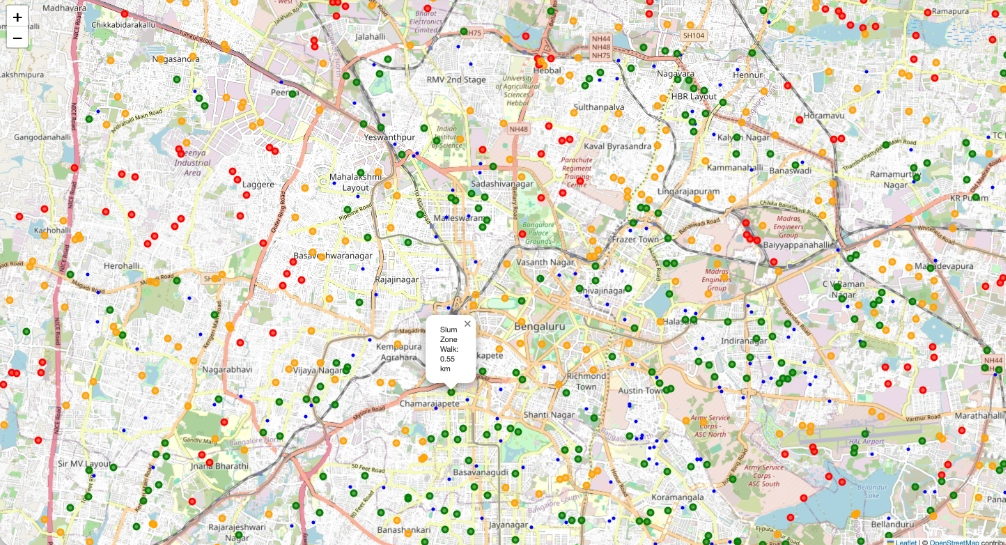
\includegraphics[width=0.8\textwidth]{vulnerability_map_slum_zone_0_55km_cropped.png}
\caption{Interactive vulnerability map of central Bengaluru (broad school filter), with an informal-zone location 0.55\km{} from the nearest government school selected. Markers show sample locations coloured by network walking distance: green $\le$1\km{}, orange 1--2\km{}, red $>$2\km{}; small blue points are schools.}
\label{fig:vmap}
\vspace{10pt}
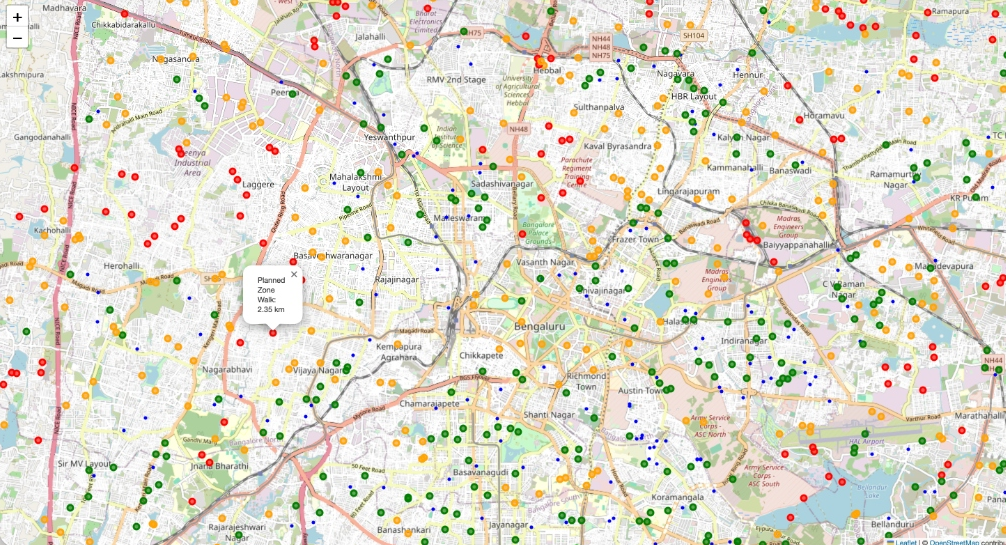
\includegraphics[width=0.8\textwidth]{vulnerability_map_planned_zone_2_35km_cropped.png}
\caption{The same vulnerability map with a planned-zone location 2.35\km{} from the nearest government school selected.}
\label{fig:vmap2}
\end{figure*}

%=====================================================================
\section{Discussion}\label{sec:discussion}
%=====================================================================
\subsection{A City-Wide Compliance Gap}
The most robust finding does not depend on the formal--informal distinction: across Bengaluru, most children cannot reach a government school within the 1\km{} walk the RTE rules promise. This holds for both classified zone types, for registered slums, and under both school definitions. Only the size of the gap changes, from roughly 60--65\% non-compliance with the broad set to over 80\% with the curated set. For the youngest children, the effective choice is between a long walk to a government school and a nearby private school.

\subsection{Planned Layouts and Privatised Substitution}
Planned layouts are, on average, slightly farther from government schools than informal areas, and they are close to dense networks of non-government schools. This pattern is consistent with \emph{privatised substitution}: where households can pay, demand shifts to private schools \cite{kingdon2020}, and there is little pressure to site government schools in planned layouts. Policy changes in Karnataka point the same way. A January 2019 amendment to Rule~4 of the Karnataka RTE Rules exempted private unaided schools from the 25\% RTE quota in neighbourhoods that have a government or aided school, and the Karnataka High Court upheld the amendment in May 2019 \cite{hc2019}. RTE-quota admissions have since been reported to have fallen from over one lakh in 2018 to 3,412 \cite{tnie2026}. Under this rule, the presence of a government school, however far away on foot, determines whether a poor child can claim a free seat in a nearby private school, which makes accurate walking-distance audits all the more consequential. Our data cannot establish causality, and the formal--informal difference we measure is small. The hypothesis that planned layouts are \emph{strongly} disadvantaged is not supported once private schools are removed from the government set.

\subsection{Invisibility as Exclusion}
The clearest equity signal in the data concerns administrative visibility. Non-notified slums are significantly farther from government schools than notified slums, and peripheral zones are the least served. These are the settlements least likely to appear in the planning frames used for conventional RTE audits. A network audit built from open data can expose this gap directly, which is the central practical argument for the pipeline.

\subsection{From Distance to Load: Re-examining the Density Penalty}
An earlier version of this work proposed a ``density penalty'' in which proximity in informal settlements is offset by overcrowding. The real data refine that idea. Settlement population and density do not predict distance. However, potential demand from slums is concentrated on a small number of government schools: ten schools are the nearest option for over 70\% of slum residents. Without open enrolment and capacity data, we cannot say whether these schools are over capacity. The load ranking nevertheless gives planners a short, concrete list of schools whose capacity should be checked first, and it can feed directly into capacity-aware measures such as 2SFCA \cite{luo2003} once capacities are known.

\subsection{Implications for Auditing Practice}
Three recommendations follow. First, compliance audits should use network distance: straight-line buffers misclassify about half of the apparently compliant locations. Second, audits should include the full slum register, not only notified slums. Third, the identity of a ``government school'' in open data needs curation; a naive keyword filter roughly halves the apparent gap.

%=====================================================================
\section{Threats to Validity and Limitations}\label{sec:validity}
%=====================================================================
\subsection{Agreement between the Classifier and KSDB Ground Truth}
The Random Forest was trained on pixels inside KSDB polygons, yet its predicted classes agree poorly with those polygons at the sample locations (Table~\ref{tab:agree}). Only 1.9\% of locations predicted informal fall inside a KSDB polygon (vs.\ 0.8\% of planned locations), and within 250\m{} or 500\m{} buffers the two classes are indistinguishable. Several factors contribute. KSDB slums are small (median 1.25\,ha, i.e., about 125 Sentinel-2 pixels), so at 10\m{} resolution many slum pixels are spectrally mixed with their surroundings, as Wurm \textit{et al.}\ \cite{wurm2019} also found. The KSDB register is also incomplete, and the model uses only five spectral features with no texture. Formal accuracy assessment on held-out labelled data was not performed. Consequently, the ``informal'' class should be read as \emph{informal-like spectral morphology}, not as verified slum. This is why we report the KSDB-based results (Section~\ref{sec:slums}) alongside the classified-sample results, and why our equity conclusions rest primarily on the former.

\begin{table}[!t]
\centering
\caption{Agreement of Classified Samples with KSDB Slum Polygons}
\label{tab:agree}
\footnotesize
\begin{tabular}{@{}lrr@{}}
\toprule
\textbf{Share of samples (\%)} & \textbf{Pred.\ informal} & \textbf{Pred.\ planned} \\
\midrule
Inside a KSDB polygon & 1.9 & 0.8 \\
Within 100\m{} of a polygon & 6.9 & 6.1 \\
Within 250\m{} of a polygon & 15.9 & 16.4 \\
Within 500\m{} of a polygon & 41.2 & 39.6 \\
\midrule
$n$ & 364 & 636 \\
\bottomrule
\end{tabular}
\end{table}

\subsection{School Data}
OSM school coverage and attributes are incomplete. Government schools that are unmapped or unnamed in OSM are missing from both sets, which biases distances upward. The curated filter trades recall for precision: it removes private ``Public'' schools but may also drop government schools whose names lack a keyword. The broad and curated results therefore bracket the plausible range. Neither set distinguishes reliably between primary and secondary levels; 49 of the 111 curated schools are explicitly primary. Because missing government schools can only lengthen measured distances, all compliance figures in this paper are best read as lower bounds on access. Official UDISE+ records would remove this uncertainty, but they could not be used to validate OSM coverage: the public UDISE+ dashboard and reports (e.g., Report~1003, schools by management and category) are disaggregated only to state level for 2025--26, reporting 74,578 schools in Karnataka of which 65.07\% are government-managed, with no district- or city-level breakdown \cite{udise2026}, and school coordinates are available only to authorised users of the UDISE+ GIS portal. The completeness of OSM's government-school layer for Bengaluru therefore cannot be quantified from open data.

\subsection{Routing Assumptions}
Distances are measured node to node; the snapping leg (median 22--47\m{}) is excluded. Polygon schools are represented by centroids rather than gates, which can over- or under-state the walk to large campuses. The OSM walk network may omit informal footpaths through settlements, which would overstate distances for informal origins, and it does not model road-crossing difficulty or safety, which would understate effective distances.

\subsection{Population Data}
WorldPop 2020 is a modelled product that disaggregates census totals using covariates, and it is known to be uncertain in dense informal areas. Slum populations here are therefore estimates. The catchment load counts all residents, not school-age children, and does not reflect actual enrolment choices.


%=====================================================================
\section{Conclusion and Future Work}\label{sec:conclusion}
%=====================================================================
This paper presented an open, reproducible pipeline for auditing the RTE walking-distance mandate. It combines Sentinel-2 classification, OSM network routing with a labelled multi-source Dijkstra search, the KSDB slum register, and WorldPop population. Applied to Bengaluru, it shows that the compliance gap is city-wide: with curated government schools, only 17.3\% of sampled locations and 20.1\% of slum residents are within a 1\km{} walk. Planned layouts are marginally farther from government schools than informal areas, but the difference is negligible in effect size and sensitive to how government schools are identified. Straight-line audits overstate compliance, with nearly half of apparently compliant locations failing on the street network. Non-notified slums and peripheral zones are the least served, and potential slum demand concentrates on a handful of government schools.

\textbf{Future work} will address the limitations above:
\begin{enumerate}
\item \textbf{Authoritative school data.} Replace name-based filtering with UDISE+ school locations, management type and level (obtained through authorised access to the UDISE+ GIS portal), and add enrolment capacities to compute capacity-aware 2SFCA accessibility.
\item \textbf{Validated classification.} Add GLCM texture \cite{haralick1973} and VHR imagery, create an independent labelled validation set, and report a proper ablation with accuracy, precision, recall and F1-score.
\item \textbf{School-age population.} Use age-structured WorldPop layers to weight by children aged 6--14 rather than all residents.
\item \textbf{Public transit.} Integrate BMTC bus stops and routes to assess whether locations beyond walking range have viable transit access to schools.
\item \textbf{Siting optimisation and dashboard.} Deploy the pipeline as an interactive planning dashboard and add location--allocation optimisation to recommend sites for new government schools that maximise population-weighted 1\km{} coverage under budget constraints.
\end{enumerate}

\section*{Acknowledgement}
The authors gratefully acknowledge PES University, Bengaluru. We thank the European Space Agency for Sentinel-2 imagery, the OpenStreetMap contributors, the WorldPop project, and the Karnataka Slum Development Board for the slum register.

\begin{thebibliography}{00}
\bibitem{census2011} Office of the Registrar General \& Census Commissioner, India, ``Census of India 2011: Provisional population totals,'' Ministry of Home Affairs, Government of India, 2011.
\bibitem{unhabitat2003} UN-Habitat, \textit{The Challenge of Slums: Global Report on Human Settlements 2003}. London, U.K.: Earthscan, 2003.
\bibitem{rte2009} Government of India, ``The Right of Children to Free and Compulsory Education Act, 2009,'' \textit{The Gazette of India}, Act No.~35 of 2009.
\bibitem{rterules2010} Ministry of Human Resource Development, Government of India, ``The Right of Children to Free and Compulsory Education Rules, 2010,'' Rule~6, 2010. [Online]. Available: \url{https://indiankanoon.org/doc/42884596/} (accessed Oct. 5, 2026).
\bibitem{drusch2012} M. Drusch \textit{et al.}, ``Sentinel-2: ESA's optical high-resolution mission for GMES operational services,'' \textit{Remote Sens. Environ.}, vol.~120, pp.~25--36, 2012.
\bibitem{gorelick2017} N. Gorelick, M. Hancher, M. Dixon, S. Ilyushchenko, D. Thau, and R. Moore, ``Google Earth Engine: Planetary-scale geospatial analysis for everyone,'' \textit{Remote Sens. Environ.}, vol.~202, pp.~18--27, 2017.
\bibitem{boeing2017} G. Boeing, ``OSMnx: New methods for acquiring, constructing, analyzing, and visualizing complex street networks,'' \textit{Comput., Environ. Urban Syst.}, vol.~65, pp.~126--139, 2017, doi: 10.1016/j.compenvurbsys.2017.05.004.
\bibitem{tatem2017} A. J. Tatem, ``WorldPop, open data for spatial demography,'' \textit{Sci. Data}, vol.~4, Art.~no.~170004, 2017, doi: 10.1038/sdata.2017.4.
\bibitem{kuffer2016} M. Kuffer, K. Pfeffer, and R. Sliuzas, ``Slums from space---15 years of slum mapping using remote sensing,'' \textit{Remote Sens.}, vol.~8, no.~6, p.~455, 2016, doi: 10.3390/rs8060455.
\bibitem{kohli2012} D. Kohli, R. Sliuzas, N. Kerle, and A. Stein, ``An ontology of slums for image-based classification,'' \textit{Comput., Environ. Urban Syst.}, vol.~36, no.~2, pp.~154--163, 2012, doi: 10.1016/j.compenvurbsys.2011.11.001.
\bibitem{mahabir2018} R. Mahabir, A. Croitoru, A. T. Crooks, P. Agouris, and A. Stefanidis, ``A critical review of high and very high-resolution remote sensing approaches for detecting and mapping slums: Trends, challenges and emerging opportunities,'' \textit{Urban Sci.}, vol.~2, no.~1, p.~8, 2018, doi: 10.3390/urbansci2010008.
\bibitem{duque2015} J. C. Duque, J. E. Patino, L. A. Ruiz, and J. E. Pardo-Pascual, ``Measuring intra-urban poverty using land cover and texture metrics derived from remote sensing data,'' \textit{Landsc. Urban Plan.}, vol.~135, pp.~11--21, 2015.
\bibitem{haralick1973} R. M. Haralick, K. Shanmugam, and I. Dinstein, ``Textural features for image classification,'' \textit{IEEE Trans. Syst., Man, Cybern.}, vol.~SMC-3, no.~6, pp.~610--621, 1973.
\bibitem{wurm2019} M. Wurm, T. Stark, X. X. Zhu, M. Weigand, and H. Taubenb\"{o}ck, ``Semantic segmentation of slums in satellite images using transfer learning on fully convolutional neural networks,'' \textit{ISPRS J. Photogramm. Remote Sens.}, vol.~150, pp.~59--69, 2019, doi: 10.1016/j.isprsjprs.2019.02.006.
\bibitem{breiman2001} L. Breiman, ``Random forests,'' \textit{Mach. Learn.}, vol.~45, no.~1, pp.~5--32, 2001.
\bibitem{belgiu2016} M. Belgiu and L. Dr\u{a}gu\c{t}, ``Random forest in remote sensing: A review of applications and future directions,'' \textit{ISPRS J. Photogramm. Remote Sens.}, vol.~114, pp.~24--31, 2016.
\bibitem{tucker1979} C. J. Tucker, ``Red and photographic infrared linear combinations for monitoring vegetation,'' \textit{Remote Sens. Environ.}, vol.~8, no.~2, pp.~127--150, 1979.
\bibitem{zha2003} Y. Zha, J. Gao, and S. Ni, ``Use of normalized difference built-up index in automatically mapping urban areas from TM imagery,'' \textit{Int. J. Remote Sens.}, vol.~24, no.~3, pp.~583--594, 2003, doi: 10.1080/01431160304987.
\bibitem{talen1998} E. Talen and L. Anselin, ``Assessing spatial equity: An evaluation of measures of accessibility to public playgrounds,'' \textit{Environ. Plan. A}, vol.~30, no.~4, pp.~595--613, 1998, doi: 10.1068/a300595.
\bibitem{luo2003} W. Luo and F. Wang, ``Measures of spatial accessibility to health care in a GIS environment: Synthesis and a case study in the Chicago region,'' \textit{Environ. Plan. B}, vol.~30, no.~6, pp.~865--884, 2003, doi: 10.1068/b29120.
\bibitem{radke2000} J. Radke and L. Mu, ``Spatial decompositions, modeling and mapping service regions to predict access to social programs,'' \textit{Geogr. Inf. Sci.}, vol.~6, no.~2, pp.~105--112, 2000, doi: 10.1080/10824000009480538.
\bibitem{hagberg2008} A. A. Hagberg, D. A. Schult, and P. J. Swart, ``Exploring network structure, dynamics, and function using NetworkX,'' in \textit{Proc. 7th Python Sci. Conf. (SciPy)}, 2008, pp.~11--15.
\bibitem{erwig2000} M. Erwig, ``The graph Voronoi diagram with applications,'' \textit{Networks}, vol.~36, no.~3, pp.~156--163, 2000.
\bibitem{okabe2008} A. Okabe, T. Satoh, T. Furuta, A. Suzuki, and K. Okano, ``Generalized network Voronoi diagrams: Concepts, computational methods, and applications,'' \textit{Int. J. Geogr. Inf. Sci.}, vol.~22, no.~9, pp.~965--994, 2008.
\bibitem{dijkstra1959} E. W. Dijkstra, ``A note on two problems in connexion with graphs,'' \textit{Numer. Math.}, vol.~1, pp.~269--271, 1959.
\bibitem{haklay2010} M. Haklay, ``How good is volunteered geographical information? A comparative study of OpenStreetMap and Ordnance Survey datasets,'' \textit{Environ. Plan. B}, vol.~37, no.~4, pp.~682--703, 2010, doi: 10.1068/b35097.
\bibitem{barrington2017} C. Barrington-Leigh and A. Millard-Ball, ``The world's user-generated road map is more than 80\% complete,'' \textit{PLoS ONE}, vol.~12, no.~8, Art.~no.~e0180698, 2017, doi: 10.1371/journal.pone.0180698.
\bibitem{kingdon2020} G. G. Kingdon, ``The private schooling phenomenon in India: A review,'' \textit{J. Dev. Stud.}, vol.~56, no.~10, pp.~1795--1817, 2020, doi: 10.1080/00220388.2020.1715943.
\bibitem{muralidharan2015} K. Muralidharan and V. Sundararaman, ``The aggregate effect of school choice: Evidence from a two-stage experiment in India,'' \textit{Q. J. Econ.}, vol.~130, no.~3, pp.~1011--1066, 2015.
\bibitem{mann1947} H. B. Mann and D. R. Whitney, ``On a test of whether one of two random variables is stochastically larger than the other,'' \textit{Ann. Math. Statist.}, vol.~18, no.~1, pp.~50--60, 1947.
\bibitem{cliff1993} N. Cliff, ``Dominance statistics: Ordinal analyses to answer ordinal questions,'' \textit{Psychol. Bull.}, vol.~114, no.~3, pp.~494--509, 1993.
\bibitem{romano2006} J. Romano, J. D. Kromrey, J. Coraggio, and J. Skowronek, ``Appropriate statistics for ordinal level data: Should we really be using t-test and Cohen's d for evaluating group differences on the NSSE and other surveys?'' in \textit{Annu. Meeting Florida Assoc. Institutional Res.}, 2006.
\bibitem{efron1993} B. Efron and R. J. Tibshirani, \textit{An Introduction to the Bootstrap}. New York, NY, USA: Chapman \& Hall, 1993.
\bibitem{udise2026} Ministry of Education, Government of India, ``UDISE+ dashboard and Report 1003: Number of schools by school management and school category, Karnataka, 2025--26.'' [Online]. Available: \url{https://dashboard.udiseplus.gov.in} (accessed Oct. 5, 2026).
\bibitem{hc2019} High Court of Karnataka, \textit{Education Rights Trust v. Government of Karnataka}, judgment of May 31, 2019. [Online]. Available: \url{https://indiankanoon.org/doc/143950994/} (accessed Oct. 5, 2026).
\bibitem{tnie2026} The New Indian Express, ``Karnataka RTE intake plunges; panel calls for age expansion,'' Feb. 21, 2026. [Online]. Available: \url{https://www.newindianexpress.com/states/karnataka/2026/Feb/21/karnataka-rte-intake-plunges-panel-calls-for-age-expansion} (accessed Oct. 5, 2026).
\end{thebibliography}

\end{document}
